\chapter{Isometric Knee Torque}\label{ch:torque}\label{ch:results}
\graphicspath{{../Figures/30-torque/}{figs/30-torque/}}

{\doublespacing\normalsize\upshape
\noindent Publication note: This chapter is the subject of an unpublished manuscript in preparation by Bolen, Burgess, Morrow, Elzein, Pang, Scharzenberger, and Hunt \citep{bolen_isometric_2025}. For that work, B.B.\ performed the conceptualization, methodology, software, validation, formal analysis, investigation, data curation, visualization, and original draft preparation; M.E., L.P., L.B., and C.M.\ contributed methodology, software, investigation, and data curation; and A.H.\ supervised the work, administered the project, and acquired funding. All co-authors contributed to writing, review, and editing.\par}

This chapter connects the actuator force characterization of Chapter~\ref{ch:muscles} to torque about the robot knee. The rigid-body torque model of the earlier robot work assumed inextensible muscle paths on rigid links, and the isometric tests reported here show where that assumption fails and by how much. The chapter proceeds from the simple pinned knee to the biomimetic joint, identifies the correction terms that remove the rigid-body idealization from the torque prediction, validates them on held-out tests, and closes with the attachment-route redesign that brings the actuator configurations to human-scaled torque targets. The methods, results, and discussion follow the manuscript noted above.

\section{Methods}

\subsection{Robot Leg Model and Knee Test Stands}\label{sec:robot_model}


The primary components of the robot leg are the knee joint, femur, tibia, BPA assemblies, and artificial tendons (Fig. \ref{fig:testJigs}\textbf{A--C}). The artificial bone components are 3D printed using a combination of Onyx, carbon fiber, and high-strength high-temperature fiberglass on Markforged Onyx One and Mark Two printers, as well as machined links for the knee mechanism. Onyx is a proprietary Markforged material that consists of chopped carbon fiber in nylon. Artificial tendons are made with Shimano bicycle brake cable.

\begin{figure}[htbp]
    \begin{center}
    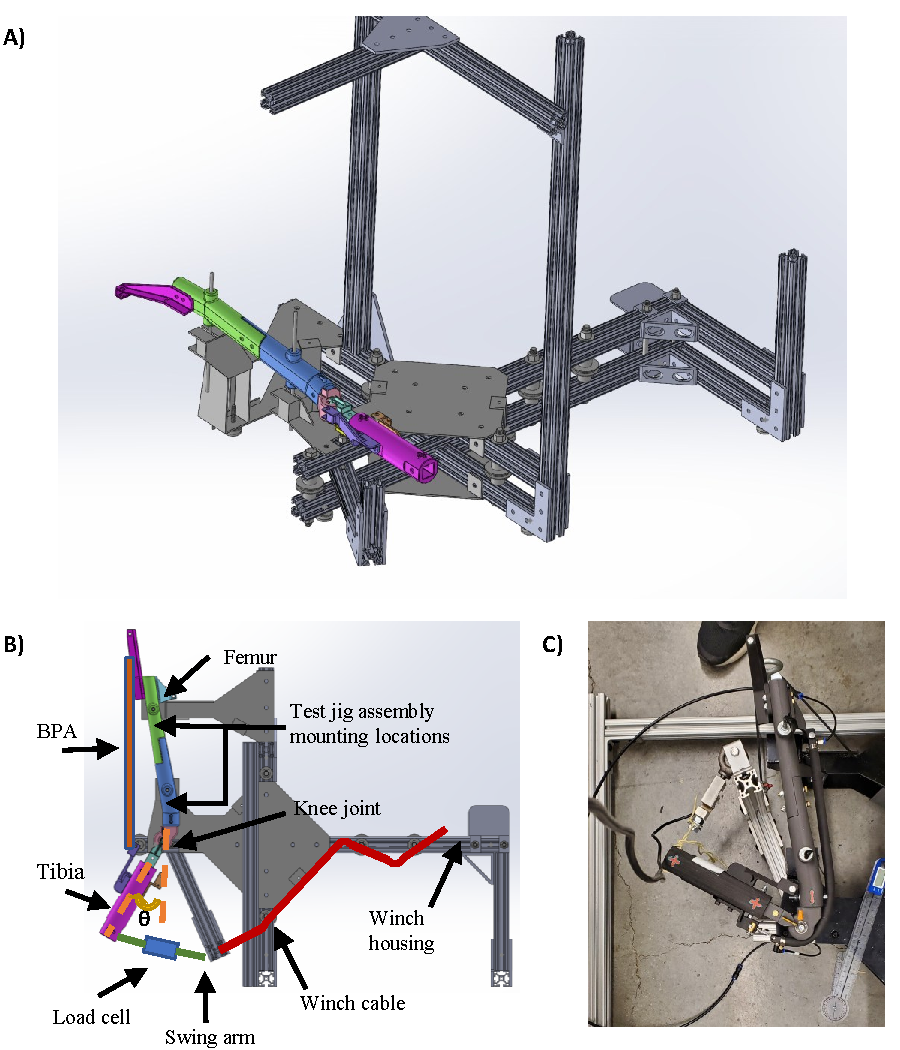
\includegraphics[width=0.73\textwidth]{testJigs_reviewed.pdf}
    \end{center}
    \caption{\textbf{(A)} CAD solid model assembly of the revolute joint knee in the test stand. \textbf{(B)} 1-DoF pinned-joint robot knee in the test apparatus with important components labeled. Leg is shown with 30 degrees flexion, i.e. $\theta_\text{k} = \ang{-30}$. \textbf{(C)} Picture from isometric torque testing. Setup shows the revolute knee configured for a test of the extensor BPA. The knee is flexed with $\theta_\text{k} = \ang{-120}$. Also note the compressed shape of the inflated BPA on the knee during this high degree of flexion. }\label{fig:testJigs}
\end{figure}

The leg assembly geometry and dimensions are based on bones scans of a $6 \, \text{ft}$  (\qty{1.83}{\metre}) tall person \citep{bolen_determination_2019,seth_opensim_2018,delp_interactive_1990,delp_opensim_2007}. Two knee joints were tested, one pure rotational joint, and one biomimetic joint with rotation and translation. Each joint is driven by two antagonistic Festo actuators. Both robot joints have the same center of rotation in the femur frame at $\theta_\text{k}=0 \deg$.

Details on the biomimetic robot knee used in this study can be found in \citep{steele_biomimetic_2018,steele_development_2017,steele_biomimetic_2018-1}. In brief, this 1-DoF joint (Fig. \ref{fig:ICR}) uses a four-bar linkage to change the effective moment arm during rotation. The intersection point of the internal crossed links define the instantaneous center of rotation (ICR). This causes the joint ICR location in the femur frame to translate posteriorly in the $X$ direction and distally in the $Y$ direction except for a brief proximal move near full flexion. Reference coordinate frames are given by \citet{wu_for_1995,wu_isb_2002}. This is similar to how the human knee behaves \citep{bolen_determination_2019,morrow_optimization_2020,seth_opensim_2018,delp_opensim_2007,delp_interactive_1990}. The correct location of the ICR is important for both theoretical and experimental torque calculations.

\begin{figure}[htbp]
    \begin{center}
    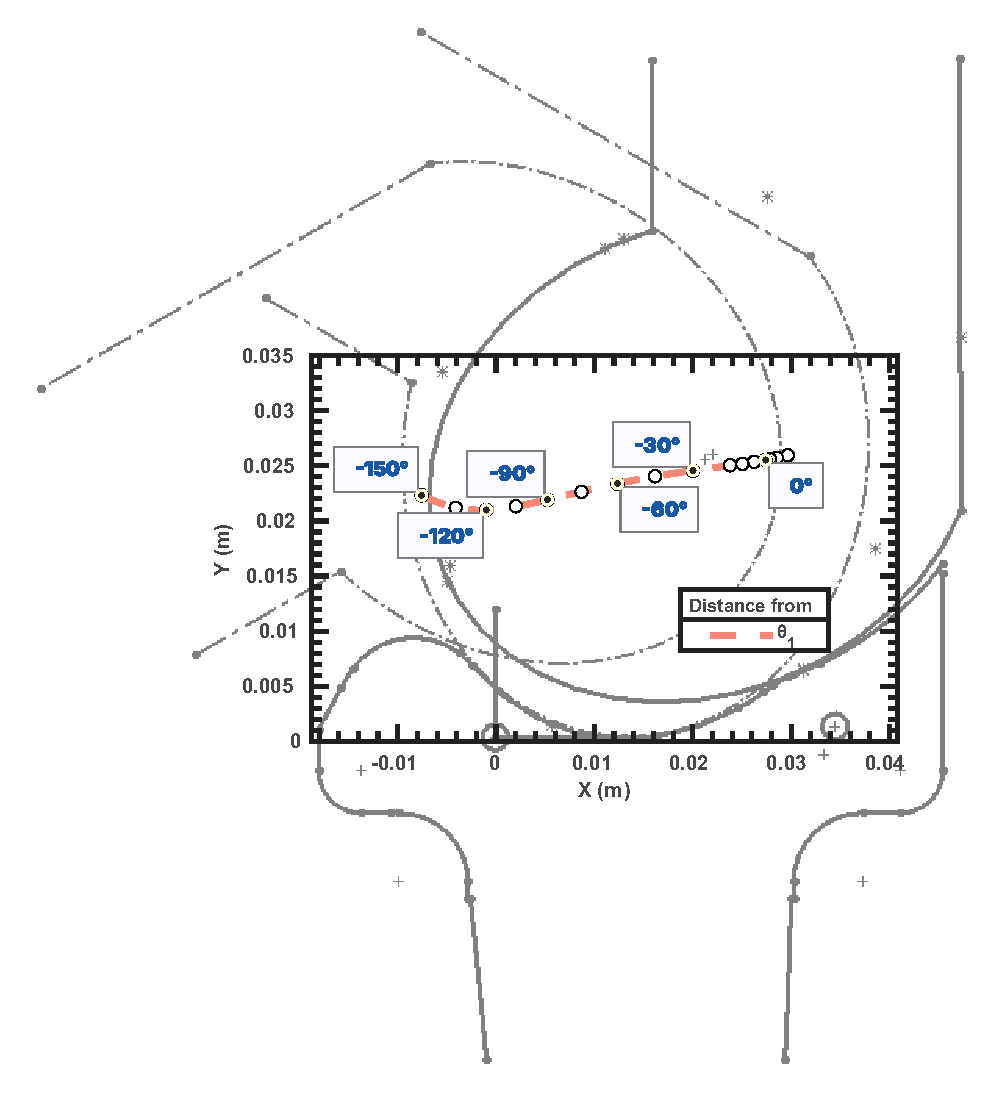
\includegraphics[width=0.8\textwidth]{KneeICR.eps}
    \end{center}
    \caption{ICR for biomimetic robot knee as a function of knee angle. Measured from $\theta_{1}$ on the tibia. Plot is overlayed on model of the knee at $\theta_\text{k}=0^\circ$ (solid line), and $-60^\circ$ and $-120^\circ$ (dotted dash lines). White circles represent measured points in $-15^\circ$ increments from $-150^\circ$ to $-15^\circ$, $-5^\circ$ increments from $-15^\circ$ to $0^\circ$, and then at $2^\circ$, $5^\circ$, and $10^\circ$.}\label{fig:ICR}
\end{figure}

Uniarticular knee extensor and knee flexor are used to actuate the joint. Each knee joint type was tested with a single $\diameter$\qty{10}{\mm} Festo BPA per muscle. The biomimetic knee was additionally tested with $\diameter$\qty{20}{\mm} Festo BPAs in a paired configuration: the extensor with two BPAs in parallel, and the flexor with two BPAs whose pathways are mirrored about the $Z$ axis. Each artificial muscle is pinned at the muscle origin location on the femur while the other end is either pinned or attached to the muscle insertion location on the tibia via an artificial tendon.

Torque about the knee is generated by the moment of the BPA force about the joint's instantaneous center of rotation (ICR). Two vectors enter that moment: the position vector $\mathbf{d}$, drawn from the ICR to the point where the actuator force is applied, and the force vector $\mathbf{F} = \norm{\mathbf{F}}\hat{\mathbf{u}}$, whose direction $\hat{\mathbf{u}}$ is the line of action of the actuator. The moment of the force about the joint is $\mathbf{m} = \mathbf{d} \times \mathbf{F}$, and its magnitude is the force magnitude multiplied by the moment arm $r$, the perpendicular distance from the joint axis to the line of action,

\begin{equation}
    r = \norm{\mathbf{d} \times \hat{\mathbf{u}}}
    \label{eq:momentarm_def}
\end{equation}

The moment arm is therefore a scalar, and it is the same quantity whether it is computed from the position vector with Eq.~\eqref{eq:momentarm_def} or measured directly with a tape measure. In this study it is calculated using the method specified by \citet{young_analyzing_2019}. The scalar moment arm $r_{k}$ about the joint axis $\hat{\mathbf{z}}_{k}$ (i.e., the $Z$ axis in the knee frame) is calculated as 

\begin{equation}
    r_{k} = \mathbf{p}_{proj,xy} \cdot \frac{\mathbf{p}_{f} \times \hat{\mathbf{z}}_{k}} { \norm{\mathbf{p}_{f} \times \hat{\mathbf{z}}_{k}} } \label{eq:project_ma}
\end{equation}

A muscle path may be modeled as a single segment running from origin to insertion, or as a chain of segments joined at via points. The segment that crosses from one reference frame into the other, here from the femur frame to the tibia frame, is the free muscle segment: because its endpoints ride on different bodies, its length and its direction respond directly to joint rotation, whereas a segment contained within one body's frame rotates rigidly with that body and changes neither. In Eq.~\eqref{eq:project_ma}, $\mathbf{p}_{proj,xy}$ is the free muscle segment projected onto the $XY$--plane, which is normal to the joint axis, and $\mathbf{p}_{f}$ is the projected muscle segment vector. Moment arm is calculated in the tibial body frame.

Details of the existing model and the torque calculation methodology in the modeled robot are given by \citet{bolen_determination_2019, morrow_optimization_2020}.

\subsection{Knee Torque Data Collection and Equipment}\label{sec:torque_equipment}


A test jig was built to collect knee torque measurements at different knee angles over its range of motion. The test stand frame is made predominantly out of 80/20 1515 series extruded aluminum components. The knee joint is free to rotate the tibia while the femur is fixed to the frame. A force sensor has one end connected to the tibia and the other is connected to a swing arm. The swing arm is tied to a winch with $3/16\; \text{inch}$ Kevlar rope from Quality Nylon Rope routed over intermediate idler pulleys (see Fig. \ref{fig:testJigs}\textbf{B} and \ref{fig:testJigs}\textbf{C}). At each measured position of $\theta_{k}$ the winch would be locked and the BPA would be inflated and then deflated. This test procedure kept the measured results as isometric as possible.  The knee joint is co-axial with gravity to eliminate gravitational torque (see Fig. \ref{fig:testJigs}\textbf{A} and Fig. \ref{fig:testJigs}\textbf{C}).

Force data was collected using one of two different sensors. The first is a MODERN STEP $\qty{300}{\kilo\gram}$ digital crane scale. The second force sensor is a CALT DYLY-103 $\qty{100}{\kilo\gram}$ S shaped load cell. The load cell is used in conjunction with a HX711 Load Cell Amplifier. Pressure is measured with a Freescale MPX5700 GP $\qty{5}{\volt}$ pressure sensor. Building air supply pressure is controlled with two pressure regulators in series. The first is a Parker model 20R113GC $0-120\; \text{psi}$ pressure regulator. The second is a Husky $3/8 \; \text{inch}$ High Performance Air Regulator HDA72200. A Festo VTUG-10-MRCR-S1T-26V20-T516LA-UL-T532S-8K valve manifold was used to supply air to the actuator. Pressure and load cell amplifier data are sent to MATLAB via an Arduino Uno style Sparkfun BlackBoard C microcontroller. 


The length measurements were made using a tape measure. When there was sufficient curvature in the BPA during knee extensor torque tests, a flexible piece of string was used to mark the axial length and then transferred to the tape measure. Angle measurements were taken with a Medigauge digital electronic goniometer or with MALENOO analog goniometers of 6, 8, or 12 inch lengths.  

\subsection{Hybrid Torque Calculation Method}\label{sec:hybrid_method}


A Hybrid Torque calculation method was developed to help uncover inconsistencies between the model and recorded torque values. This method measures the actual muscle length and angles of the robot to calculate force and joint torque. With this method, it is easier to determine which parts of the torque equation did not achieve their predicted value and provide a correction to that part of the equation. The classical mechanics way to calculate the torque about a joint is to take the cross product of the position vector $\mathbf{d}$ and the force vector $\mathbf{F}$, both defined in Section~\ref{sec:robot_model},

\begin{equation}
    \mathbf{m} = \mathbf{d} \times \mathbf{F} \label{eq:M_vec}
\end{equation}

Knee torque is the scalar component of this moment about the joint axis, written $M_{z}$ to make its axis explicit. Because the moment arm is the perpendicular distance from that axis to the line of action, the vector cross product of Eq.~\eqref{eq:M_vec} reduces to an ordinary scalar product,

\begin{equation}
    M_{z} = r\,F \label{eq:M_scalar}
\end{equation}

where $r$ is the scalar moment arm of Eq.~\eqref{eq:momentarm_def}, here measured directly with a tape measure as the perpendicular distance from the knee axis to the actuator's line of action, and $F$ is the scalar force magnitude, calculated by measuring the BPA's $P$, $l_{0}$, $l_{620}$ and $l_\text{m}$ values and using the model fit equations determined in the following section. The hybrid method therefore replaces the model-predicted moment arm $r_{k}$ of Eq.~\eqref{eq:project_ma} and the model-predicted muscle length with their measured counterparts, leaving the force model as the only predicted quantity.

\subsection{Improved Torque Model}\label{sec:improved_model}

The classical kinematic torque model assumed rigid links and inextensible muscle paths. Data collected during the first flexor experiments (Section~\ref{sec:results_torque}) showed that this assumption does not hold for a pneumatic system: measured muscle lengths were consistently shorter than predicted, and measured torque deviated from prediction in a load-dependent manner. This section describes the corrections that were developed to account for a constant length offset, series compliance in the attachment hardware and artificial tendons, and the loss of usable muscle length when a BPA wraps around the joint.

These corrections are deliberately formulated to be identified from experiment rather than derived analytically, because the physical effects they represent are distributed and not separately measurable. The lumped compliance absorbs the cantilevered three-dimensional-printed attachment brackets, whose geometry is a printed CAD part rather than a prismatic beam with a tractable second moment of area, together with the bone fixtures, the cable winch of the test stand, and the artificial tendon. Predicting that aggregate stiffness from first principles would require finite-element models of each component with material properties (anisotropic printed polymer, braided sleeve, construction-dependent tendon stiffness) that are themselves unmeasured. The correction terms therefore parameterize only what the torque model needs: $\chi_{0}$ absorbs the constant length discrepancy observed at zero load, $\chi_{1}$ and $\chi_{2}$ are effective stiffnesses in the bracket frame's principal directions, and $\chi_{3}$ scales the wrapping-length loss. Each is identified by global optimization against the measured torque rather than solved in closed form, for two reasons. First, the terms enter the prediction through an implicit force balance, because the compliance displacement depends on the force that it itself modifies, so the inverse problem has no analytic solution. Second, the parameters are only jointly identifiable: preliminary fits showed that widely different stiffness pairs can reproduce the training tests nearly equally well, so the adopted solution must be selected by cross-validated prediction on held-out tests rather than by residual minimization alone, which is what the multiobjective Pareto-front procedure of Section~\ref{sec:optimization} provides.

\subsubsection{Length Offset and System Stiffness}\label{sec:offset_stiffness}

Analysis of measured muscle length data shows that it was consistently shorter than the predicted muscle length at all joint angles. This shorter length results in less muscle force, a shifted RoM, and less torque in the experimental setup. That this shorter length occurs when $\varepsilon=1$ and $F=0$ indicates that a constant length offset should be used. Therefore, to produce an improved torque prediction model, $l_\text{m}$ was recalculated as

\begin{equation}
    l_\text{m} = l_{LMT} - 2\;l_{fitting} - \chi_{0} 
    \label{eq:Lm}
\end{equation}

where $l_{LMT}$ is the path length of the musculotendon from origin to insertion point, $l_{fitting}$ is the length of the end caps, and $\chi_{0}$ is a constant length offset. 

Additionally, as the muscles produce more force, compliant components in the limb segments and attachment hardware deform. This deformation changes the effective braided pneumatic actuator (BPA) length, which alters contraction and therefore changes the force predicted by the BPA model. This effect is most apparent at high forces and low contractions. The purpose of the compliance model developed next is predictive, not structural: it exists so that the torque calculation can correct the actuator length for load-dependent deformation, and it makes no claim about the stiffness of any one component in isolation. Accordingly, the stiffness values that populate the model, $\chi_{1}$ and $\chi_{2}$, are not measured on the hardware directly; they are identified by the optimization of Section~\ref{sec:optimization} from the measured torque, and every stiffness value quoted later in this chapter is an optimizer output. The combined hardware compliance is approximated using Hooke's law in the bracket's principal directions.

A local bracket frame was established at the attachment bracket. The $\hat{\mathbf{x}}_{br}$ axis was aligned with the vector from the bracket reference point to the BPA attachment point and represents the stiffest direction of the bracket. The $\hat{\mathbf{y}}_{br}$ axis was chosen to point in the posterior direction with respect to the tibia frame, corresponding to the primary cantilever bending direction (see Fig.~\ref{fig:bktFrame}), while the $\hat{\mathbf{z}}_{br}$ axis completes the right-handed frame. In this frame the bracket is modeled as three independent linear springs along the principal axes, with stiffnesses $k_{x}$, $k_{y}$, and $k_{z}$ in the $x_{br}$, $y_{br}$, and $z_{br}$ directions.

For the two-rotation evaluator, the bracket frame was constructed from the vector joining the bracket origin to attachment point $\mathbf{p}_{A}$ or $\mathbf{p}_{B}$. The first rotation, through $\theta_z$ about the fixed space-frame axis $\hat{\mathbf{z}}_{s}$, points the intermediate axis $\hat{\mathbf{x}}_{1}$ toward the sagittal-plane projection, $\mathbf{p}_{A}^{\mathrm{sag}}$ for the insertion point $\mathbf{p}_{A}$ and $\mathbf{p}_{B}^{\mathrm{sag}}$ for the origin point $\mathbf{p}_{B}$. The second rotation, through $-\theta_y$ about the current axis $\hat{\mathbf{y}}_{1}=\hat{\mathbf{y}}_{br}$, brings the final bracket axis $\hat{\mathbf{x}}_{br}$ into alignment with the full three-dimensional point vector. Figure~\ref{fig:xiFrameTransform} shows these geometric targets. The resulting orientation and homogeneous transform are

\begin{equation}
\mathbf{R}_{sb}=\mathbf{R}_z(\theta_z)\mathbf{R}_y(\theta_y)^T,
\qquad
\mathbf{T}_{sb}=
\begin{bmatrix}
\mathbf{R}_{sb} & \mathbf{p}_{br}\\
\mathbf{0}^{T} & 1
\end{bmatrix}.
\label{eq:bracket_frame_transform}
\end{equation}

\begin{figure}[htbp]
\centering
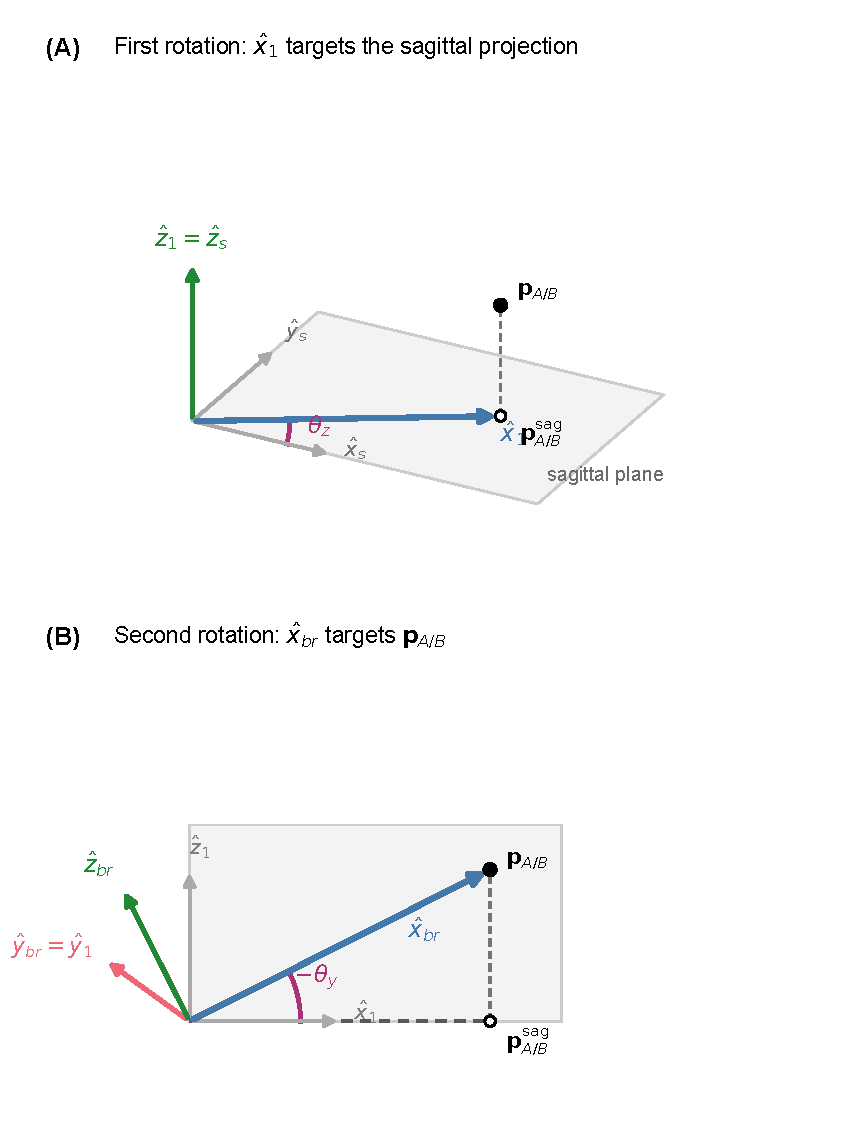
\includegraphics[height=0.72\textheight]{xiFrameTransform.pdf}
% ALT TEXT: Two vertically stacked diagrams construct the local bracket frame.
% Panel A rotates about the fixed space z axis until the intermediate x axis
% points toward the sagittal-plane projection of attachment point pA or pB.
% Panel B rotates about the current y axis until the final bracket x axis points
% directly toward the full three-dimensional attachment point.
\caption[Two-rotation construction of the bracket frame]{Two-rotation construction of the bracket frame from attachment point $\mathbf{p}_{A}$ or $\mathbf{p}_{B}$. \textbf{(A)} Rotation through $\theta_z$ about fixed $\hat{\mathbf{z}}_{s}$ aligns $\hat{\mathbf{x}}_{1}$ with the point's sagittal-plane projection. \textbf{(B)} Rotation through $-\theta_y$ about current $\hat{\mathbf{y}}_{1}=\hat{\mathbf{y}}_{br}$ aligns $\hat{\mathbf{x}}_{br}$ with the full point vector.}
\label{fig:xiFrameTransform}
\end{figure}

\begin{figure}[htbp]
\begin{center}
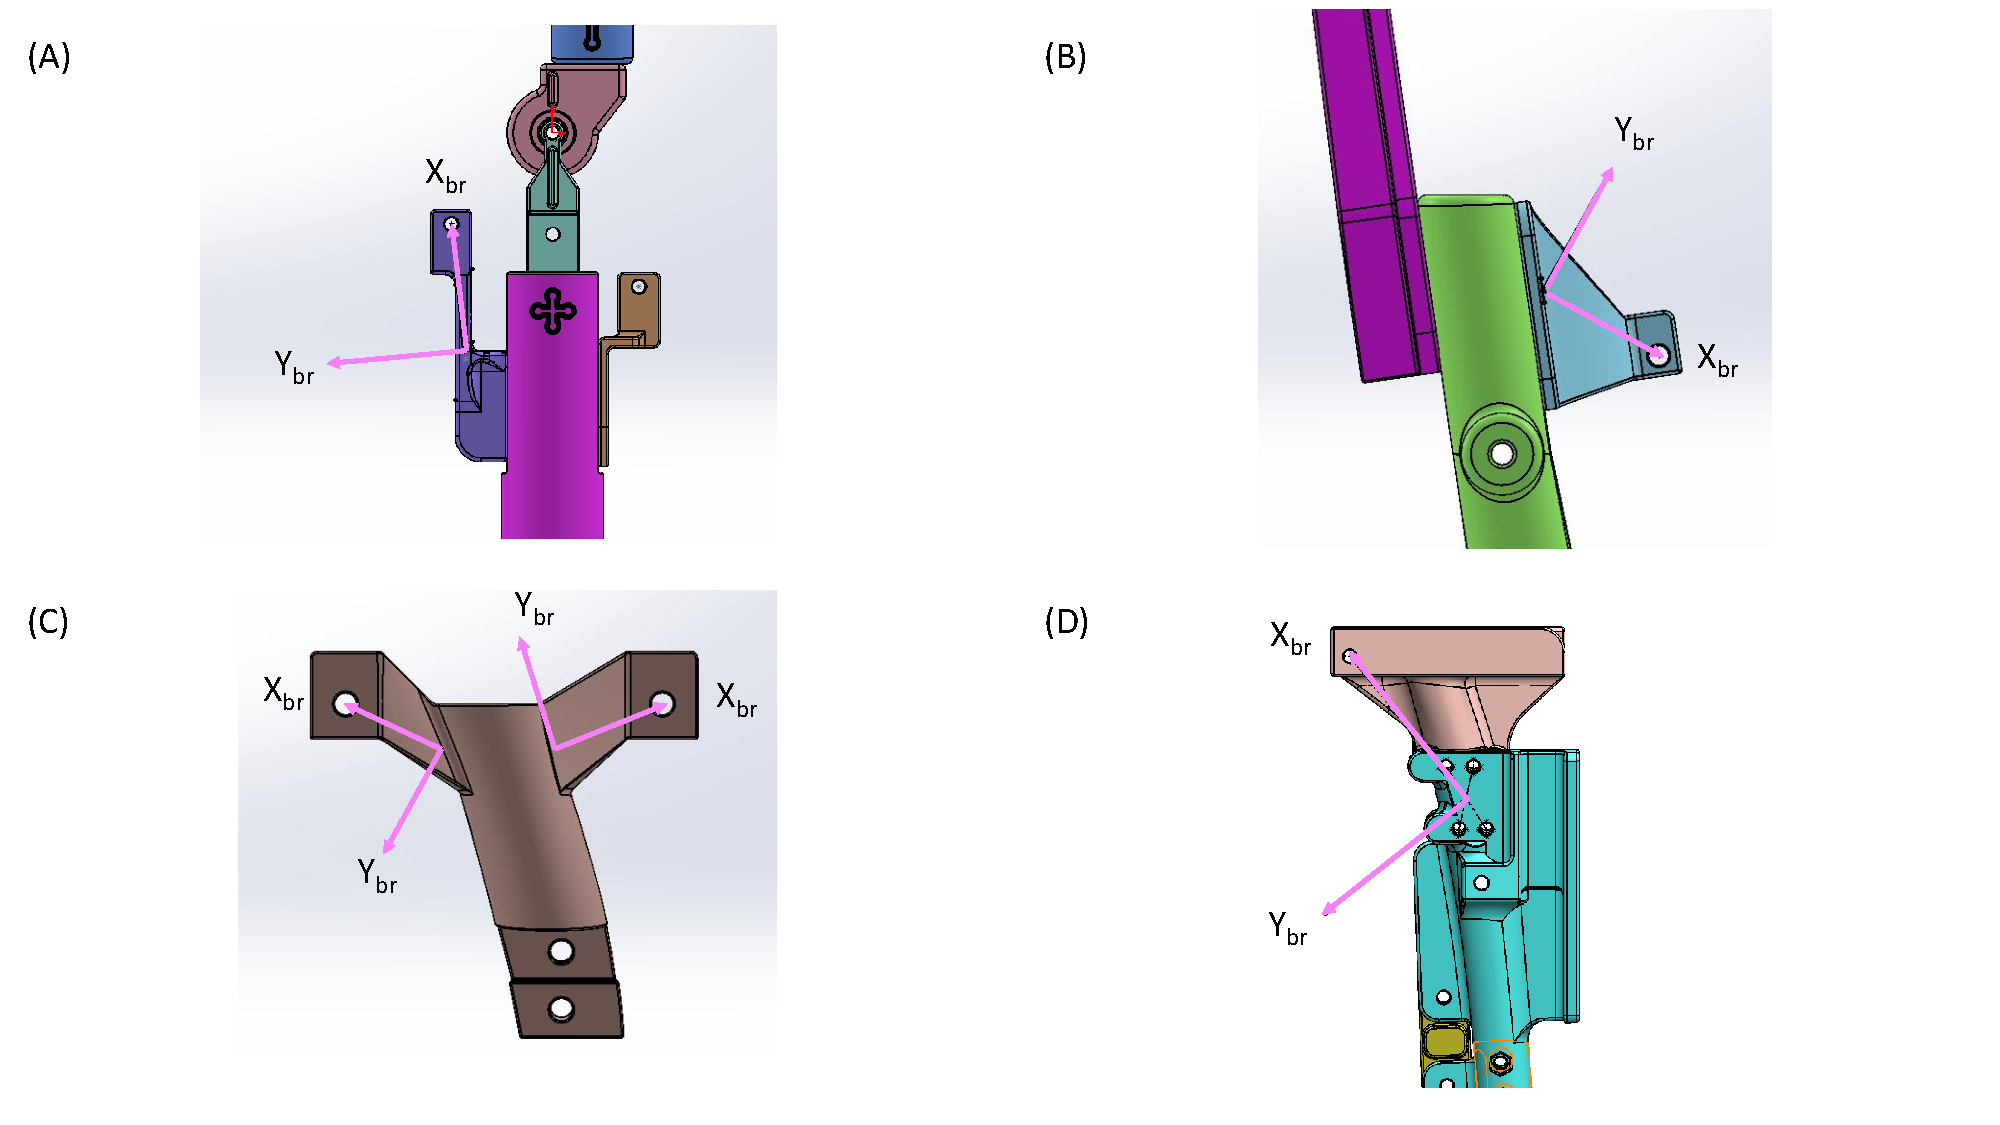
\includegraphics[width=1\textwidth]{bktFrame.pdf}
\end{center}
\caption{Bracket frame orientations for: \textbf{(A)} flexor configuration on the pinned knee, \textbf{(B)} extensor configuration on the pinned knee, \textbf{(C)} flexor and extensor configurations on the biomimetic knee with $\diameter$\qty{10}{\mm} BPAs, and \textbf{(D)} flexor configuration on the biomimetic knee with the $\diameter$\qty{20}{\mm} BPA.}
\label{fig:bktFrame}
\end{figure}

\begin{equation}
\mathbf{K}_{br} = \operatorname{diag}\!\left(k_{x},\; k_{y},\; k_{z}\right)
\label{eq:bktstiffness_general}
\end{equation}

These three principal stiffnesses are not independent in this model, and the reason follows from the frame construction itself. The first rotation of Eq.~\eqref{eq:bracket_frame_transform} is fixed by the sagittal-plane projection of the attachment point, but the orientation of the bracket frame about its own $\hat{\mathbf{y}}_{br}$ axis is a modeling choice: the pitch-only convention (no second rotation) and the two-rotation convention of Fig.~\ref{fig:xiFrameTransform} describe the same physical bracket and differ by exactly a rotation about $\hat{\mathbf{y}}_{br}$. A diagonal stiffness array is invariant under such a rotation, $\mathbf{R}_{y}(\theta)\,\mathbf{K}_{br}\,\mathbf{R}_{y}(\theta)^{T} = \mathbf{K}_{br}$ for all $\theta$, if and only if the two stiffnesses in the plane of the rotation are equal, $k_{x} = k_{z}$. Adopting this y-symmetric form therefore makes the compliance prediction independent of the frame convention, and the redundant third stiffness is eliminated: with this array the two frame conventions produce identical torque predictions to numerical precision.

The change of notation that follows is deliberate. The symbols $k_{x}$, $k_{y}$, and $k_{z}$ name the stiffness components of the general bracket-frame array, Eq.~\eqref{eq:bktstiffness_general}; $\chi_{1}$ and $\chi_{2}$ are the two identified stiffness parameters, the quantities the optimization of Section~\ref{sec:optimization} solves for, and each enters the diagonal array in a fixed axis assignment. Two stiffness values remain, $\chi_{1}$ in the $x_{br}$ and $z_{br}$ directions and $\chi_{2}$ in the cantilever bending direction $y_{br}$:

\begin{equation}
\mathbf{K}_{br} = 
\begin{bmatrix}
\chi_{1} & 0   & 0 \\
0   & \chi_{2} & 0 \\
0   & 0   & \chi_{1} \\
\end{bmatrix}
\label{eq:bktstiffness}
\end{equation}

The corresponding local compliance matrix is 

\begin{equation}
\mathbf{C}_{br} = \mathbf{K}_{br}^{-1}
\label{eq:bktcompliance}
\end{equation}

The force applied to the bracket was expressed in the bracket frame as $\mathbf{F}_{br}$. This force vector can be written in terms of its magnitude and unit direction as

\begin{equation}
\mathbf{F}_{br} = F \, \hat{\mathbf{u}}
\label{eq:bktforcevector}
\end{equation}
\noindent
where $F = \norm{\mathbf{F}}$ is the scalar force magnitude of Eq.~\eqref{eq:M_scalar} and $\hat{\mathbf{u}} = [u_{x}, u_{y}, u_{z}]^{T}$ is the BPA force direction expressed in the bracket frame. The bracket deflection vector, $\boldsymbol{\epsilon}_{br}$, was calculated from Hooke's law as 

\begin{equation} \mathbf{F}_{br} = \mathbf{K}_{br} \: \boldsymbol{\epsilon}_{br}
\label{eq:bktvectorhooke}
\end{equation}

Solving Eq. \ref{eq:bktvectorhooke} for the bracket deflection gives

\begin{equation}
\boldsymbol{\epsilon}_{br} = \mathbf{K}_{br}^{-1} \: \mathbf{F}_{br} = \mathbf{C}_{br} \: \mathbf{F}_{br}
\label{eq:bktdeflection}
\end{equation}

Substituting Eq. \ref{eq:bktforcevector} into Eq. \ref{eq:bktdeflection} gives

\begin{equation}
\boldsymbol{\epsilon}_{br} = F \,\mathbf{K}_{br}^{-1} \,\hat{\mathbf{u}}
\label{eq:bktdeflectionforceunit}
\end{equation}

For the diagonal stiffness matrix in Eq. \ref{eq:bktstiffness}, Eq. \ref{eq:bktdeflection} is equivalent to the component-wise expression

\begin{equation}
\boldsymbol{\epsilon}_{br} = \begin{bmatrix} F\,u_{x}/\chi_{1} \\ F\,u_{y}/\chi_{2} \\ F\,u_{z}/\chi_{1} \end{bmatrix}
\label{eq:bktcomponentdeflection}
\end{equation}

Although $\boldsymbol{\epsilon}_{br}$ is a three-dimensional deflection vector, the BPA force model depends on the scalar change in effective BPA length ($\delta$). Therefore, only the component of $\boldsymbol{\epsilon}_{br}$ along the BPA line of action directly changes the effective BPA length. This scalar bracket deflection is the projection of $\boldsymbol{\epsilon}_{br}$ onto $\hat{\mathbf{u}}$:

\begin{equation}
{\delta}_{br} = \hat{\mathbf{u}}^{T} \boldsymbol{\epsilon}_{br}
\label{eq:bktprojecteddeflection}
\end{equation}

Substituting Eq. \ref{eq:bktdeflection} into Eq. \ref{eq:bktprojecteddeflection} gives

\begin{equation}
{\delta}_{br} = \hat{\mathbf{u}}^{T} \, \mathbf{K}_{br}^{-1} \, \mathbf{F}_{br}
\label{eq:bktprojecteddeflection2}
\end{equation}

Using Eq. \ref{eq:bktforcevector}, Eq. \ref{eq:bktprojecteddeflection2} becomes

\begin{equation}
\delta_{br} = F\, \hat{\mathbf{u}}^{T} \, \mathbf{K}_{br}^{-1} \, \hat{\mathbf{u}}
\label{eq:bktprojectedcompliance}
\end{equation}

The scalar stiffness along the BPA line of action due to the bracket compliance is therefore

\begin{equation}
k_{\hat{u},br} = \frac{F}{\delta_{br}} = \left( \hat{\mathbf{u}}^{T} \mathbf{K}_{br}^{-1} \hat{\mathbf{u}} \right)^{-1}
\label{eq:keff}
\end{equation}

This projected-compliance form is used because the force is applied along $\hat{\mathbf{u}}$, while the bracket is allowed to deflect independently along its local $\hat{\mathbf{x}}_{br}$, $\hat{\mathbf{y}}_{br}$, and $\hat{\mathbf{z}}_{br}$ directions. The reduced-order Hooke's law expression for the bracket deflection along the BPA line of action is therefore

\begin{equation} F = k_{eq} \: \delta
\label{eq:hookereduced}
\end{equation}

Here $k_{eq}$ is the series sum of every compliant element in the actuator path, and the bracket-only case is the special case with no tendon. When the BPA attaches directly to the bracket, $k_{eq}$ excludes the tendon and equals $k_{\hat{u},br}$ of Eq.~\eqref{eq:keff}. When an artificial tendon was used, it was modeled as an axial spring with stiffness $k_{ten}$: bracket deflection and tendon stretch both shorten the effective BPA length along the actuator line of action, the two elements carry the same force, and their scalar compliances add in series,

\begin{equation} k_{eq} = \left( \frac{1}{k_{\hat{u},br}} + \frac{1}{k_{ten}} \right)^{-1}
\label{eq:equivalentstiffness}
\end{equation}

This series reduction is exact only under a specific set of conditions, each of which corresponds to a way the physical hardware could violate it. The bracket and the tendon must carry the same force, which holds for two massless elements coupled in series under quasi-static loading; a compliant coupling between them would break this. Their displacements must be kinematically additive along the line of action, with no displacement lost to off-axis geometry. Within a single iteration of the force balance the line of action $\hat{\mathbf{u}}$ is treated as fixed, which is an approximation, and one the results justify: once the balance returns the compliance displacement, the calculation updates the attachment locations with the deflected bracket positions and re-evaluates $\hat{\mathbf{u}}$ and the moment arm at the deflected geometry, as described below. The elements are assumed to carry no moment, so rotational compliance and force--moment coupling at the attachments are neglected. Both elements are linear, with stiffness independent of deflection, and the tendon is modeled without preload, so its tangent stiffness does not stiffen with load state. Finally, compliance deflection shortens the actuator, as Eq.~\eqref{eq:activelengthcorrected} assumes, because a BPA produces force only in tension: under its own pulling force the compliant attachments give way in the direction that relieves that tension. A deflection that would lengthen the actuator can be produced by an antagonistic pull, but that loading lies outside this treatment.

Since $\delta$ is the scalar compliance displacement along the BPA line of action, then the compliance-corrected active BPA length used in the force balance is

\begin{equation} l_m(\delta) = l_m{(0)} - \delta
\label{eq:activelengthcorrected}
\end{equation}

where $l_m{(0)}$ is the initial muscle length calculated from \eqref{eq:Lm}.

For a specified set of correction parameters, the following calculation solves the attachment-compliance displacement at each knee angle; it is distinct from the optimization that identifies those parameters from experimental torque data (Section~\ref{sec:optimization}). The corresponding relative contraction is $\varepsilon^*(\delta)$. Since the BPA force depends on contraction, and contraction depends on the compliance displacement, $\delta$ is the root of the nonlinear force-balance equation

\begin{equation} F_{\mathrm{max}} \cdot F_{\mathrm{BPA}}\!\left(\varepsilon^*(\delta),P^*\right) - k_{eq}\,\delta = 0
\label{eq:complianceforcebalance}
\end{equation}

The root is found with a bracketed scalar solver (\texttt{fzero} in MATLAB) on the physically admissible interval between zero deflection and the deflection that would bring the actuator to its maximum usable contraction. Termination is controlled by the bracket, not by a residual tolerance: the iteration closes in on the root and stops when the bracket has collapsed to adjacent floating-point values, so the returned $\delta$ is converged to machine precision. Two safeguards act as secondary stop conditions. If the actuator already sits at or beyond its maximum usable contraction at zero deflection, no root is sought and $\delta$ is set to zero; if the residual shows no sign change across the interval, the solver likewise returns $\delta = 0$ rather than a spurious root.

After solving Eq. \ref{eq:complianceforcebalance}, the corresponding force magnitude was used in Eq. \ref{eq:bktdeflection} to compute the vector bracket deflection. This deflection was transformed back into the limb reference frame and used to update the BPA attachment location. The routed BPA length, force direction, moment arm, and torque were then recalculated using the updated attachment location. In the present implementation, the optimized stiffness terms $\chi_{1}$ and $\chi_{2}$ were treated as effective compliance parameters for the attachment system rather than direct measurements of an isolated bracket. This allowed unmodeled compliance in the surrounding hardware to be represented by the reduced-order stiffness model.

The actuator path can carry compliant hardware at both ends: the insertion-side bracket of the preceding development together with a second, origin-side bracket. Figure~\ref{fig:xiProjection} distinguishes the three-dimensional displacement of each bracket from the scalar displacement along the BPA force path. For bracket $j$, the displacement resolves into components $\eta_{1,j}$, $\eta_{2,j}$, and $\eta_{3,j}$ along the local bracket-frame basis, whereas only its projection $\delta_{br,j}$ along the corresponding force direction $\hat{\mathbf{u}}_j$ changes the actuator length. The two bracket projections act in series with the tendon elongation $\delta_{\mathrm{tendon}}$:

\begin{equation}
\begin{aligned}
\boldsymbol{\eta}_{br,j} &= \sum_{i=1}^{3}\eta_{i,j}\hat{\mathbf{e}}_i^{(j)},\\
\delta_{br,j} &= \hat{\mathbf{u}}_j^T\boldsymbol{\eta}_{br,j}, \qquad j\in\{1,2\},\\
\delta_{\mathrm{series}} &= \delta_{br,1}+\delta_{\mathrm{tendon}}+\delta_{br,2}.
\end{aligned}
\label{eq:bracket_series_projection}
\end{equation}

\begin{figure}[htbp]
\centering
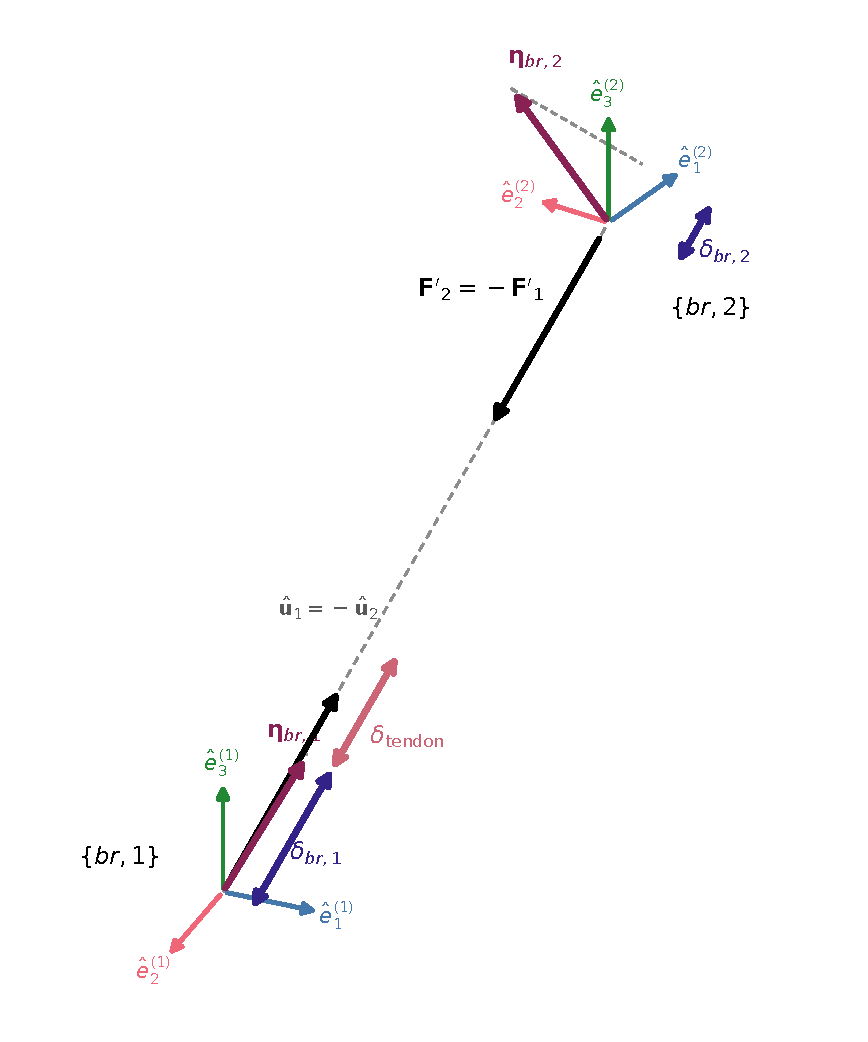
\includegraphics[height=0.72\textheight]{xiProjection.pdf}
\caption[Two-bracket deflection and force-path projection]{Two-bracket deflection and projection along the BPA force path. The force vectors at $\{br,1\}$ and $\{br,2\}$ point toward one another and satisfy $\mathbf{F}_2=-\mathbf{F}_1$. The bracket projections $\delta_{br,1}$ and $\delta_{br,2}$ are offset from the corresponding coordinate frames for clarity, and tendon elongation $\delta_{\mathrm{tendon}}$ continues collinearly from $\delta_{br,1}$. Colors follow a color-vision-deficiency-safe palette and are redundant with labels and line weights.}
\label{fig:xiProjection}
\end{figure}





\subsubsection{BPA Fictive Contraction}\label{sec:fictive_contraction}

The extensor configuration required one further correction, for a loss with a different physical origin than the compliance terms. As the knee flexes, the extensor BPA bends over the front of the joint and makes contact with it, so part of the actuator follows the joint surface instead of a straight line. Bent over the joint this way, the BPA behaves like a beam: the pressurized wall on the inside of the bend carries less tension than the wall on the outside, which both unbalances the actuator's force and consumes part of the wrapped arc length that would otherwise shorten the path. The wrapped section therefore stops contributing usable contraction length, and the actuator behaves as if it were more contracted than it physically is. This excess is termed fictive strain: the additional contraction the force model must see to reproduce the observed force, beyond the actuator's physical contraction. A wrapping-loss term $\chi_{3}$ was introduced to scale the length that this fictive strain removes, such that
\begin{equation}
    \Delta l = \begin{cases}
     \chi_{3}\;R\;\abs{ \theta_\text{wrap}-\theta_\text{k}}\;\zeta^2 & \theta_\text{k} \leq      \theta_\text{wrap} \\
      0 & \theta_\text{k} \geq \theta_\text{wrap}
     \end{cases}\label{eq:deltaL}
\end{equation}

where $\Delta l$ is the change in usable length of the BPA, $R$ is the wrapping radius, $\abs{\theta_\text{wrap}-\theta_\text{k}}$ is the angle through which the BPA is bent once contact begins, and $\theta_\text{wrap}$ is the knee flexion angle at which the BPA starts to bend over the knee joint, determined from solid modeling. $\zeta$ is the additive complement to relative strain, such that

\begin{equation}
    \zeta = 1-\varepsilon^*  \\
\label{eq:comp}
\end{equation}

so the wrapping loss grows quadratically as the actuator approaches its resting length and vanishes at full contraction. Combining \eqref{eq:comp} into \eqref{eq:deltaL}, and subtracting $\Delta l$ from  \eqref{eq:Lm} yields

\begin{equation}
    l_\text{m} = l_{LMT} - 2\;l_{fitting}  - \chi_{0} - \Delta l\label{eq:x3}
\end{equation}

\subsubsection{Multiobjective Identification Algorithm}\label{sec:identification}

Multiobjective optimization using \texttt{gamultiobj} in MATLAB was used to determine the length offset ($\chi_{0}$) and the stiffness terms ($\chi_{1}$ and $\chi_{2}$). The error between the model and the experimental torque was minimized across the pinned-knee flexor tests, with the $l_{0}=\qty{45.7}{\cm}$ test held out for validation.

The optimization algorithm was again \texttt{gamultiobj} in MATLAB. This time, the muscle origins bracket was chosen. The bracket frame is shown in Fig. \ref{fig:bktFrame}\textbf{B}. Since the bracket forms an arch shape and extends for \qty{75}{\mm} in the $Z$ direction, for this configuration, we set $\chi_{2}$ in the $X_{br}$ direction, and $\chi_{1}$ in the $Y_{br}$ and $Z_{br}$ directions. The optimization algorithm for this set solves for the best average goodness-of-fit (GoF) measures RMSE, FVU, and maximum absolute residual for two BPAs, while the third one was held out. Three independent rounds of optimization were performed, so that one of each of the BPAs could be held out as validation. The solution was then selected by the shortest distance between the average normalized GoF and the validation data, subject to improved GoF values for all the individual BPAs, with the exception of maximum absolute residual on the $l_{0}=\qty{48.0}{\cm}$ BPA.

This initial identification was subsequently extended to the full test sets in two stages. First, the flexor model was given a second compliant bracket at the origin-side attachment (a hip-frame cantilever carrying the BPA origin), so that the compliance of both ends of the actuator path is represented; the stiffness pair $(\chi_{1}, \chi_{2})$ is shared by the two brackets in fixed axis assignments (Appendix~\ref{app:model_geometry}, Table~\ref{tab:app_stiffness_arrays}), leaving a three-term fit $(\chi_{0}, \chi_{1}, \chi_{2})$ cross-validated over the four remaining flexor tests, two of them held out per fold; the encoder-corrected $l_{0}=\qty{47.9}{\cm}$ test was not used in the two-bracket identification. Second, the extensor refit locked $(\chi_{1}, \chi_{2})$ at the flexor-identified values, enforcing a single stiffness pair across the flexor and extensor configurations, and solved only the extensor-specific terms $(\chi_{0}, \chi_{3})$ on a three-test training set with three tests held out for validation, with the extensor length offset allowed to take negative values. The bounds and the adopted values of both stages are recorded in Appendix~\ref{app:model_geometry} (Tables~\ref{tab:app_opt_bounds} and~\ref{tab:app_xi_values}); the fit outcomes are summarized in Tables~\ref{tab:FlxPinGof} and~\ref{tab:ExtPinGof}.

The goodness-of-fit metrics used to judge the optimization results are the root mean square error (RMSE), the fraction of variance unexplained (FVU), and the maximum absolute residual, each computed between the measured and predicted isometric torque over the tested range of motion.

Each metric isolates a different aspect of disagreement between the two curves. RMSE reports the overall magnitude of the error and, when the curve shapes already agree, is dominated by the remaining level offset. FVU normalizes the error variance by the variance of the measured torque, making it scale-free: it asks whether the prediction reproduces the variation of the measurement rather than whether it is close in absolute units, is the complement of the Nash--Sutcliffe model efficiency \citep{nash_river_1970}, and takes values below one when the prediction outperforms the mean of the measurement itself. The maximum absolute residual is a worst-case local measure. A small shift of the predicted curve along the knee-angle axis produces large pointwise residuals where the torque gradient is steep and small residuals elsewhere, so this metric is sensitive to phase misalignment while responding only weakly to uniform level offsets.

This interpretation follows the standard decomposition of curve-comparison error into offset, amplitude, and pattern components \citep{taylor_summarizing_2001}: the mean square error between two curves separates into the squared mean offset, an amplitude mismatch, and a residual shape term. An equivalent three-term formulation, splitting waveform similarity into offset, amplitude, and shape, underlies the linear fit method developed for clinical gait waveform comparison \citep{iosa_assessment_2014}. The metrics used here map onto this decomposition, with RMSE carrying the level disagreement, FVU the shape and amplitude agreement, and the maximum absolute residual serving as the phase-sensitive worst case. FVU is treated as the primary criterion because it is the only one of the three that is directly comparable across tests with different torque scales.

\subsection{Optimization Algorithms and Cost Functions}\label{sec:optimization}

Optimization enters this chapter in several places, and in every one of them it replaces a calculation that cannot be carried out any other way. The correction terms of the improved torque model are quantities that no instrument measures directly: they are hidden inside an implicit force balance, and their best values are the ones that make the model's predicted torque match the measured torque. The route redesign is the mirror problem: the attachment locations are free design variables, and their best values are the ones that make the redesigned routes meet or exceed human torque capability. The cam-profile variant of the extensor route extends the redesign once more, searching over the shape of the tibial-side routing itself. In each case a search algorithm proposes candidate values, the physics model evaluates them, and the search proceeds until a stopping rule is met. This section states what is searched for, which solvers were chosen and why, and when each search stops.

Two families of optimization problem underpin the results of this dissertation and the design framework built on them. The first is the identification of the correction terms of Section~\ref{sec:improved_model} ($\chi_{0}$, $\chi_{1}$, $\chi_{2}$, and $\chi_{3}$) from the pinned-knee test data. The second is the redesign of the biomimetic knee route geometry, meaning the BPA origin $\mathbf{p}_{1}$, insertion $\mathbf{p}_{\text{end}}$, resting length, and tendon length (Appendix~\ref{app:model_geometry}), so that the flexor and extensor configurations meet or exceed human knee torque capability over the range of motion, together with its cam-profile extension, in which the tibial-side route points are free to trace a cam profile (Section~\ref{sec:route_redesign_results}). Both are carried out in MATLAB \citep{mathworks_optimization_2025}.

The correction-term identification is a genuine multiobjective problem: candidate parameter sets are judged simultaneously on RMSE, FVU, and maximum absolute residual (Section~\ref{sec:improved_model}). It is solved with the genetic multiobjective solver \texttt{gamultiobj}, an implementation of the elitist nondominated-sorting genetic algorithm NSGA-II \citep{deb_nsga2_2002, mathworks_optimization_2025}, which returns a Pareto front of parameter sets from which the adopted solution is selected by the holdout-validation procedure described above. The production runs use adaptive-feasible mutation and scattered crossover at a fraction of 0.8, with MATLAB's default Pareto fraction of 0.35; the population settings are stage-specific. The flexor two-bracket fit evolves a population of 150 for up to 600 generations and terminates early once the geometric average relative change in the spread of the Pareto front falls below $4\times10^{-3}$; the extensor refit uses a population of 50 for up to 150 generations with a spread tolerance of $1\times10^{-3}$. In both stages the parameters are searched in a normalized space, with length offsets in centimeters and stiffnesses on a base-ten logarithmic scale, so that the genetic search samples the stiffness bounds, which span an order of magnitude, uniformly by decade, and the initial population is seeded around the expected solution region. The search bounds and the adopted values are recorded in Appendix~\ref{app:model_geometry}.

The route redesign replaces the multiobjective formulation with a single scalar cost assembled from weighted penalty terms, because the route prediction (contact activation, wrapping, and compliance correction) is expensive to evaluate and only moderately smooth. The cost has the form
\begin{equation}
    J = w_{w}\,J_{\text{worst}} + w_{t}\,J_{\text{torque}} + \textstyle\sum_{a} J_{a} + J_{\text{geom}} + J_{\text{len}},
    \label{eq:opt_cost}
\end{equation}
where $J_{\text{worst}}$ is the largest fraction by which robot torque falls short of the human target at any angle across the range of motion, weighted heavily ($w_{w} = 10^{5}$); $J_{\text{torque}}$ is the mean-squared shortfall fraction ($w_{t} = 10^{3}$), weighted two orders of magnitude below the worst-angle term so that no shortfall at a single angle can be traded away for a better average; the $J_{a}$ are configuration-specific auxiliary penalties described below; and $J_{\text{geom}}$ and $J_{\text{len}}$ are regularizers that keep the endpoints and actuator lengths near their seed values. Human torque targets are computed from the Gait2392 lower-extremity model \citep{delp_opensim_2007, seth_opensim_2018}: the flexor is graded against the biceps femoris short head and the extensor against vastus medialis. Each target is a maximum-isometric torque curve: OpenSim moment arms, obtained as the partial derivative of muscle-tendon length with respect to the knee coordinate, $r(\theta_{k}) = \partial l_{\mathrm{MT}}/\partial\theta_{k}$, are evaluated across the range of motion and multiplied by each muscle's maximum isometric force (provenance and exported tables in Appendix~\ref{app:muscle_calcs}). Hard constraints (bone clearance, wrap feasibility, actuator strain and contraction limits, tendon geometry) are enforced alongside the cost, and any candidate whose prediction fails is rejected with a prohibitive penalty.

The solution pipeline is common to both configurations. Each run begins with a full sanity evaluation of the seed design and a small smoke test of the solver setup, then executes \texttt{surrogateopt}, MATLAB's surrogate-assisted global solver for expensive black-box objectives, which builds a spatial interpolation surrogate over sampled candidate points and searches it adaptively \citep{mathworks_optimization_2025}, in parallel under per-configuration evaluation budgets of 3,000 for the extensor route and 1,000 for the flexor route (the later cam variant of Section~\ref{sec:route_redesign_results} uses 1,000 surrogate and 1,500 refinement evaluations), and finally refines the best feasible point with \texttt{patternsearch}, a derivative-free mesh-adaptive direct search method \citep{audet_mads_2006, mathworks_optimization_2025}, for 15,000 further evaluations. The surrogate budgets sit well past the observed plateau of a few hundred evaluations, so they cap run time rather than define convergence. Each stage stops on its evaluation budget; the pattern search also stops early when its mesh collapses below the mesh tolerance with the constraints satisfied, which is the usual exit once the design has converged. The entry scripts and their cost functions are archived with the code.

Although both configurations share this pipeline, their cost functions differ in ways that reflect the mechanics. The flexor BPA routes around a single moving wrap point, so clearance from the tibia and femoral condyles is enforced by continuous signed-distance constraints, and its cost adds an off-axis torque penalty (torques about the joint axes other than the knee axis, relative to the original single-BPA route) and a penalty if the wrap fails to release cleanly as the knee extends. The extensor BPA wraps over the front of the joint through as many as seven sequential contacts, so clearance is enforced instead by the contact-elimination rule that governs the route, and its cost penalizes torque overshoot above the human curve and excessive actuator contraction, which risks bottoming out at high flexion. The flexor and extensor targets alike carry a required torque margin of 5\,\% above the human curve, so that a route that merely touches the target at any angle is rejected. With two BPAs per joint, the flexor route is mirrored about the mid-sagittal plane and the two actuator forces are summed, while the extensor model scales the force of a single shared route by the actuator count.

\section{Results}\label{sec:results_torque}

With the actuator force model validated at the actuator level, the same model was used to predict isometric torque about the knee joint for the test stands described in Sections~\ref{sec:robot_model} and~\ref{sec:hybrid_method}. Measured torque is compared against three predictions: the original rigid-body torque model of Section~\ref{sec:bg_knee}, a prediction using the improved BPA force characterization alone (Chapter~\ref{ch:muscles}), and the improved torque model of Section~\ref{sec:improved_model} after optimization. The hybrid torque method (Section~\ref{sec:hybrid_method}) is used to isolate the sources of error.

\subsection{Flexor on Pin Joint}

Figure~\ref{fig:FlxPin_preopt} shows the measured flexor torque on the pinned knee next to the pre-optimization prediction series for the four cross-validation tests. Both pre-optimization force models overpredicted the magnitude of the measured flexor torque, and on the angles where the two predictions are both defined the improved BPA characterization fit the measurements better than the original rigid-body prediction on every test, although it degraded near full extension, where the rigid-body prediction is undefined altogether (Table~\ref{tab:FlxPinPreGof}). The back-calculated (hybrid) torque reproduced the measurements closely, which localizes the misprediction to the modeled kinematics, the muscle length $l_\text{m}$ and the moment arm $r$, rather than to the force model.

\begin{figure}[htbp]
\begin{center}
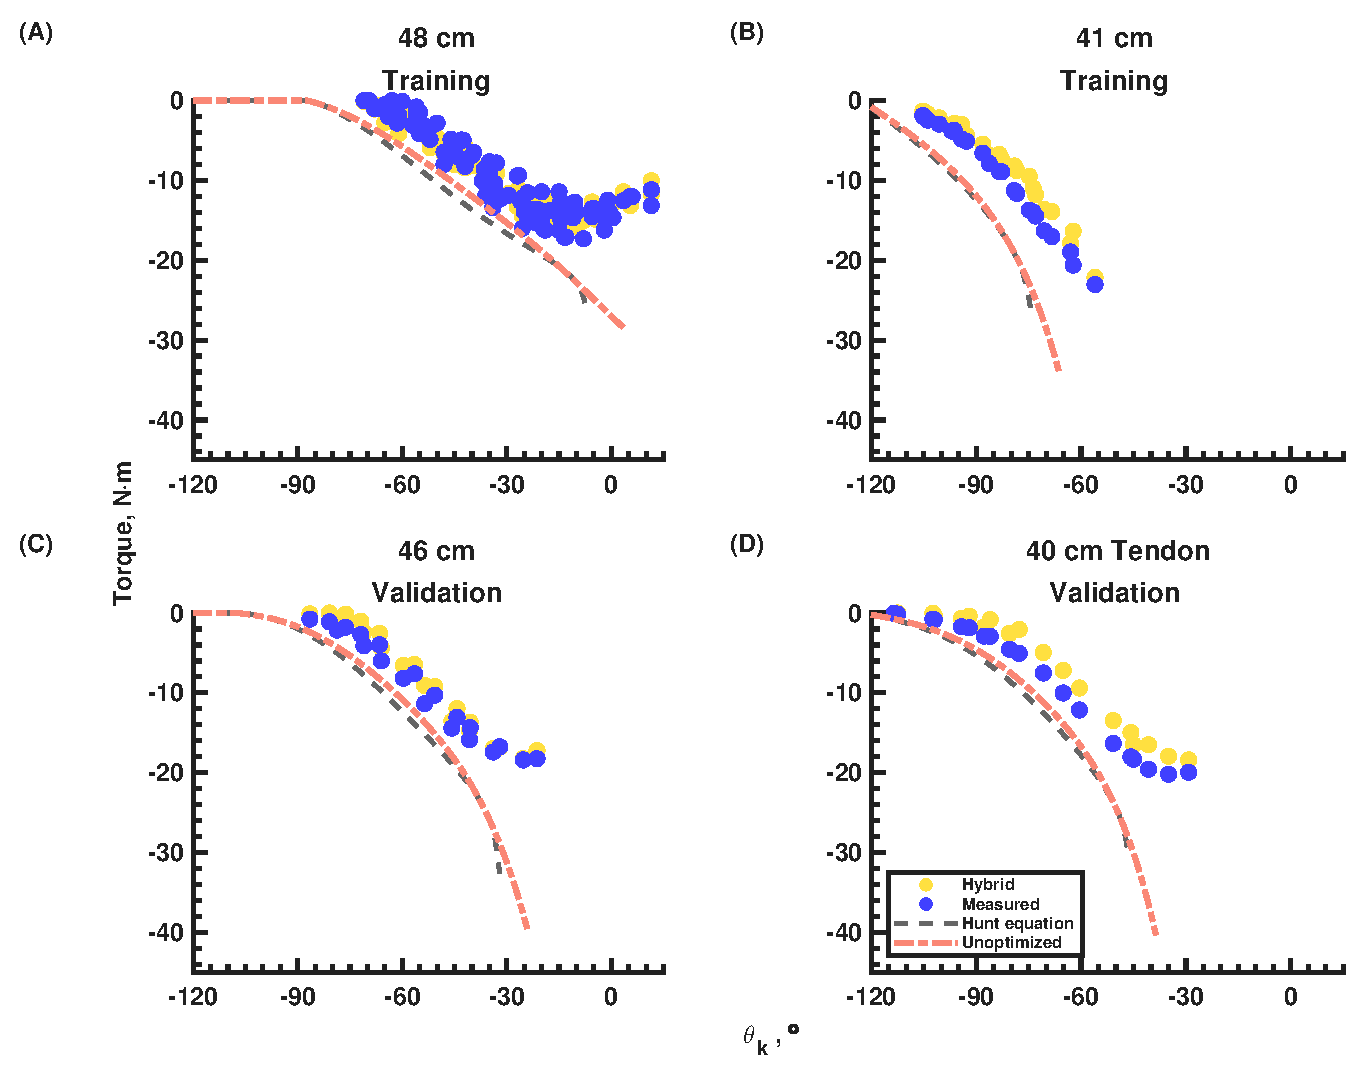
\includegraphics[width=0.9\textwidth]{FlxPin_preopt.eps}
\end{center}
\caption{Pre-optimization pinned-knee torque versus knee angle for the four cross-validation flexor tests. Knee angle is negative in flexion, and flexion torque is negative. Gold circles are the hybrid calculation, which combines the measured muscle length and moment arm with the modeled force; indigo filled circles are experimentally measured torque; the gray dashed line is the rigid-body prediction; and the light orange dash-dot line is the unoptimized prediction, the improved BPA force characterization applied to the same rigid kinematics. Panel titles give the nominal resting length; the actual resting lengths are $l_{0}=\qty{48.5}{\cm}$ \textbf{(A)}, $l_{0}=\qty{41.0}{\cm}$ \textbf{(B)}, $l_{0}=\qty{45.7}{\cm}$ \textbf{(C)}, and $l_{0}=\qty{40.6}{\cm}$ with tendon \textbf{(D)}. Panels \textbf{(A)} and \textbf{(B)} are the training tests and panels \textbf{(C)} and \textbf{(D)} the validation tests of the adopted cross-validation fold.}\label{fig:FlxPin_preopt}
\end{figure}

\begin{table}[htbp]
\caption{Pre-optimization pinned-knee flexor torque-prediction goodness of fit per test, comparing the three pre-optimization torque predictions of Figure~\ref{fig:FlxPin_preopt}: the rigid-body prediction, the unoptimized prediction of the improved BPA characterization, and the back-calculated (hybrid) torque. The rigid-body prediction is undefined near full extension, where its modeled strain falls below zero, so the rigid-body and improved-characterization columns are scored head-to-head on the measured points of each test at which the rigid-body prediction is defined (75 of 90, 17 of 20, 14 of 19, and 15 of 22 points, in panel order); the back-calculated torque is scored on all measured points. RMSE and maximum absolute residual (Max.) are in $\text{N}\cdot\text{m}$, and FVU denotes the fraction of variance unexplained. Training and validation follow the adopted cross-validation fold.}
\label{tab:FlxPinPreGof}
\fontsize{10pt}{12pt}\selectfont
\begin{tabular}{@{}lccccccccc@{}}
\toprule
& \multicolumn{3}{c}{\textbf{Rigid body}} & \multicolumn{3}{c}{\textbf{Improved char.\ alone}} & \multicolumn{3}{c}{\textbf{Back-calculated (hybrid)}} \\
\cmidrule(lr){2-4} \cmidrule(lr){5-7} \cmidrule(l){8-10}
\textbf{Test} & \textbf{RMSE} & \textbf{FVU} & \textbf{Max.} & \textbf{RMSE} & \textbf{FVU} & \textbf{Max.} & \textbf{RMSE} & \textbf{FVU} & \textbf{Max.} \\
\midrule
$l_{0}=\qty{48.5}{\cm}$ (training)           & 5.779 & 1.1761 & 9.798 & 4.871 & 0.8354 & 9.865 & 1.635 & 0.0991 & 3.842 \\
$l_{0}=\qty{41.0}{\cm}$ (training)           & 6.633 & 3.2313 & 11.409 & 6.074 & 2.7090 & 9.262 & 2.187 & 0.1184 & 4.243 \\
$l_{0}=\qty{45.7}{\cm}$ (validation)         & 5.315 & 0.9408 & 9.991 & 4.465 & 0.6640 & 9.536 & 1.246 & 0.0409 & 2.275 \\
$l_{0}=\qty{40.6}{\cm}$, tendon (validation) & 3.945 & 0.6750 & 7.527 & 3.226 & 0.4512 & 7.376 & 2.085 & 0.0755 & 3.073 \\
\midrule
Mean (training)                             & 6.206 & 2.2037 & 10.604 & 5.472 & 1.7722 & 9.563 & 1.911 & 0.1088 & 4.043 \\
Mean (validation)                           & 4.630 & 0.8079 & 8.759 & 3.845 & 0.5576 & 8.456 & 1.666 & 0.0582 & 2.674 \\
\bottomrule
\end{tabular}
\end{table}

The initial identification, fitted on the $l_{0}=\qty{48.5}{\cm}$ test, yielded a length offset $\chi_{0} = \qty{11.9}{\mm}$ and effective stiffnesses $\chi_{1} = \qty{102}{\kN\per\m}$ and $\chi_{2} = \qty{10.6}{\kN\per\m}$. The corrected model at these terms followed the measured torque across the range of motion, including the loss of torque near full extension that the rigid-body prediction did not produce, and Figure~\ref{fig:FlxPin_optimized} shows this corrected-family behavior at the adopted two-stage terms. The $l_{0}=\qty{45.7}{\cm}$ actuator, configured to operate over a different joint range of motion, served as the validation test of the initial fit; the corrected prediction reproduced the measured torque there without refitting. At these initial terms, the corrected prediction for the training test had a root-mean-square error (RMSE) of \qty{1.616}{\newton\meter}, a fraction of variance unexplained (FVU) of 0.0958, and a maximum absolute residual of \qty{3.2527}{\newton\meter}; validation on the held-out actuator gave \qty{2.1214}{\newton\meter}, 0.0878, and \qty{5.1690}{\newton\meter}, respectively (Table~\ref{tab:TorqueFit}).

\begin{figure}[htbp]
\begin{center}
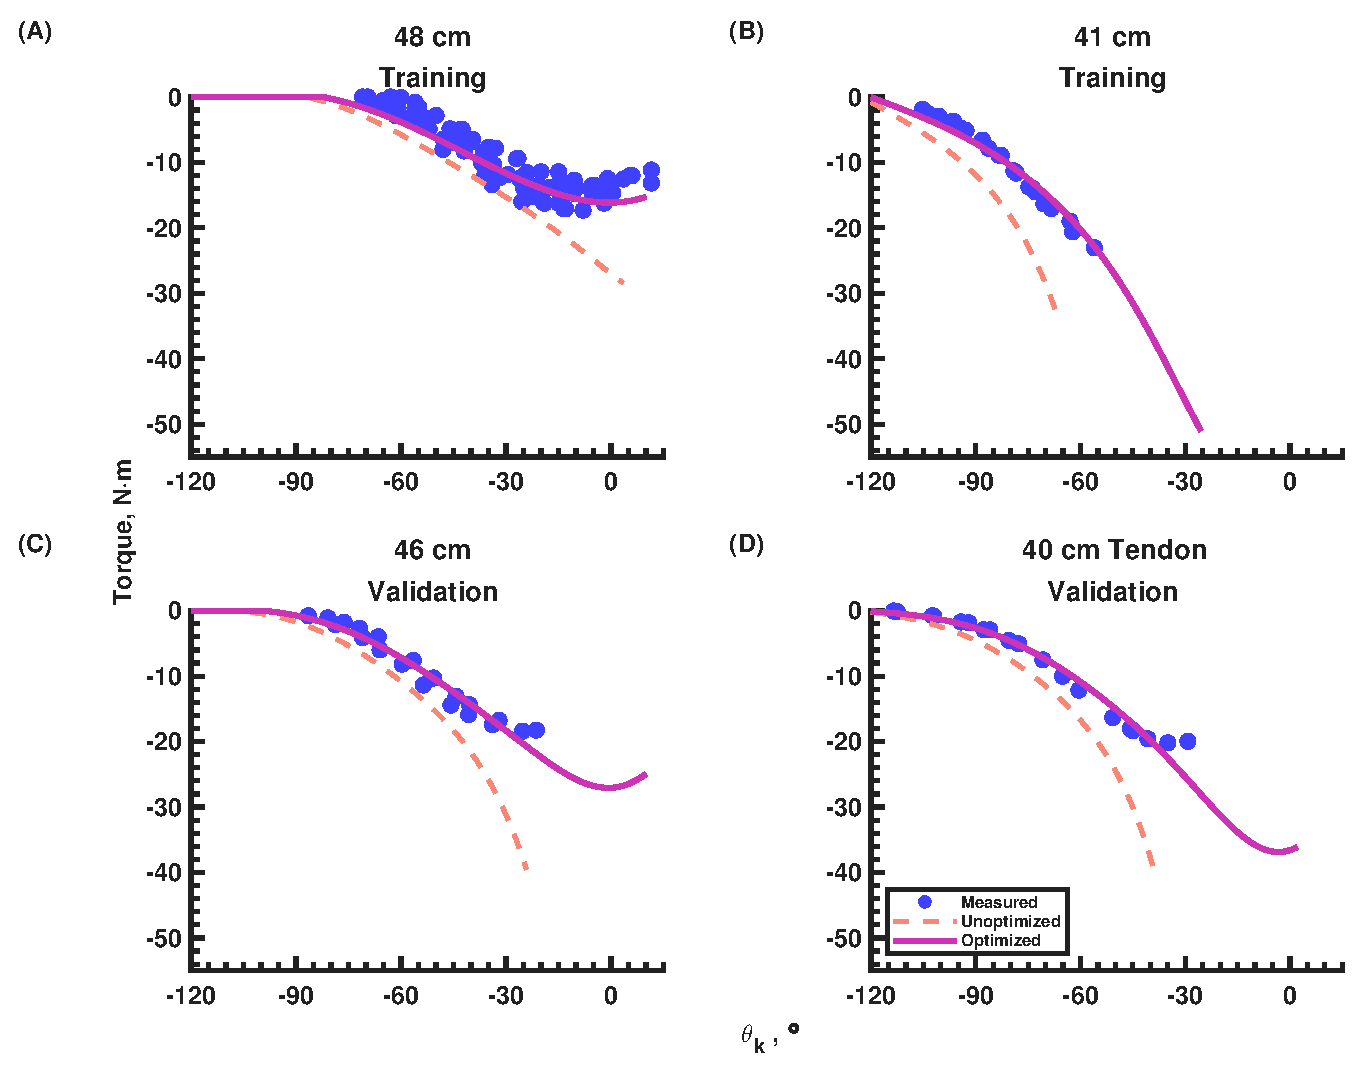
\includegraphics[width=0.9\textwidth]{FlxPin_optimized.eps}
\end{center}
\caption{Optimized pinned-knee torque versus knee angle for the four cross-validation flexor tests, at the adopted correction terms (Table~\ref{tab:AdoptedXi}). Knee angle is negative in flexion, and flexion torque is negative. Blue filled circles are experimentally measured torque; the dashed light orange line is the unoptimized prediction of the improved BPA characterization; the magenta line is the optimized prediction of the corrected model. Panel titles give the nominal resting length; the actual resting lengths are $l_{0}=\qty{48.5}{\cm}$ \textbf{(A)}, $l_{0}=\qty{41.0}{\cm}$ \textbf{(B)}, $l_{0}=\qty{45.7}{\cm}$ \textbf{(C)}, and $l_{0}=\qty{40.6}{\cm}$ with tendon \textbf{(D)}. Panels \textbf{(A)} and \textbf{(B)} are the training tests and panels \textbf{(C)} and \textbf{(D)} the validation tests of the adopted cross-validation fold; the goodness-of-fit values are given in Table~\ref{tab:FlxPinGof}.}\label{fig:FlxPin_optimized}
\end{figure}

Table~\ref{tab:FlxPinGof} completes this comparison at the adopted correction terms of the full re-identification (Section~\ref{sec:identification}). Across the four tests of the two-bracket identification, the corrected model reduces the training-mean RMSE, over the $l_{0}=\qty{48.5}{\cm}$ and \qty{41.0}{\cm} training tests, from \qty{8.66}{\newton\cdot\meter} under the zero-correction prediction, the same kinematics and force model with every correction term disabled, to \qty{1.62}{\newton\cdot\meter}, and the validation mean over the held-out $l_{0}=\qty{45.7}{\cm}$ and \qty{40.6}{\cm} tendon tests improves from \qty{7.59}{\newton\cdot\meter} to \qty{1.49}{\newton\cdot\meter}. The behavior of the original rigid-body torque model on these tests is shown graphically in Fig.~\ref{fig:FlxPin_preopt}.

\begin{table}[htbp]
\caption{Pinned-knee flexor torque-prediction goodness of fit per test. The zero-correction prediction uses the improved BPA force characterization alone (rigid attachments, no length offset, and no wrapping loss); the corrected model adds the adopted correction terms of the two-stage identification (Section~\ref{sec:identification}). RMSE and maximum absolute residual (Max.) are in $\text{N}\cdot\text{m}$. In the adopted cross-validation fold the $l_{0}=\qty{48.5}{\cm}$ and \qty{41.0}{\cm} tests formed the training set and the $l_{0}=\qty{45.7}{\cm}$ and \qty{40.6}{\cm} tendon tests were held out for validation; the $l_{0}=\qty{47.9}{\cm}$ test was not used in the identification and is reported in Appendix~\ref{app:model_geometry}.}
\label{tab:FlxPinGof}
\begin{tabular}{@{}lcccccc@{}}
\toprule
& \multicolumn{3}{c}{\textbf{Improved BPA char.\ alone}} & \multicolumn{3}{c}{\textbf{Corrected model}} \\
\cmidrule(lr){2-4} \cmidrule(l){5-7}
\textbf{Test} & \textbf{RMSE} & \textbf{FVU} & \textbf{Max.} & \textbf{RMSE} & \textbf{FVU} & \textbf{Max.} \\
\midrule
$l_{0}=\qty{48.5}{\cm}$ (training)    & 7.617 & 2.1278 & 25.531 & 2.165 & 0.1718 & 5.467 \\
$l_{0}=\qty{41.0}{\cm}$ (training)    & 9.694 & 2.1149 & 21.076 & 1.084 & 0.0277 & 1.766 \\
$l_{0}=\qty{45.7}{\cm}$ (validation)  & 8.803 & 1.9380 & 26.264 & 1.368 & 0.0468 & 3.614 \\
$l_{0}=\qty{40.6}{\cm}$, tendon (validation) & 6.373 & 0.5935 & 16.859 & 1.611 & 0.0427 & 5.891 \\
\midrule
Mean (training)                       & 8.656 & 2.1213 & 23.303 & 1.624 & 0.0998 & 3.616 \\
Mean (validation)                     & 7.588 & 1.2657 & 21.562 & 1.490 & 0.0447 & 4.752 \\
\bottomrule
\end{tabular}
\end{table}

\subsection{Extensor on Pin Joint}

When the new stiffness and length offset model was used to predict torque for the knee extensor, measured torque was slightly higher than the original rigid-body model predicts for the \qty{48.0}{\cm} resting length BPA, slightly lower than expected for the \qty{45.7}{\cm} BPA, and much lower for the \qty{41.5}{\cm} BPA. Only the $\chi_{1}$ and $\chi_{2}$ terms from the previous optimization results were used with the extensor configuration. By inspection, the zero point of the measured torque was shifted to the right of the original model, indicating an offset opposite in sign to the $\chi_{0}$ term in the previous section. The BPA with $l_{0}=\qty{45.7}{\cm}$ illustrates the pattern: the hybrid-method calculated torque correlates well with the originally predicted torque, while the actual measured torque diverges. 

\begin{figure}[htbp]
\begin{center}
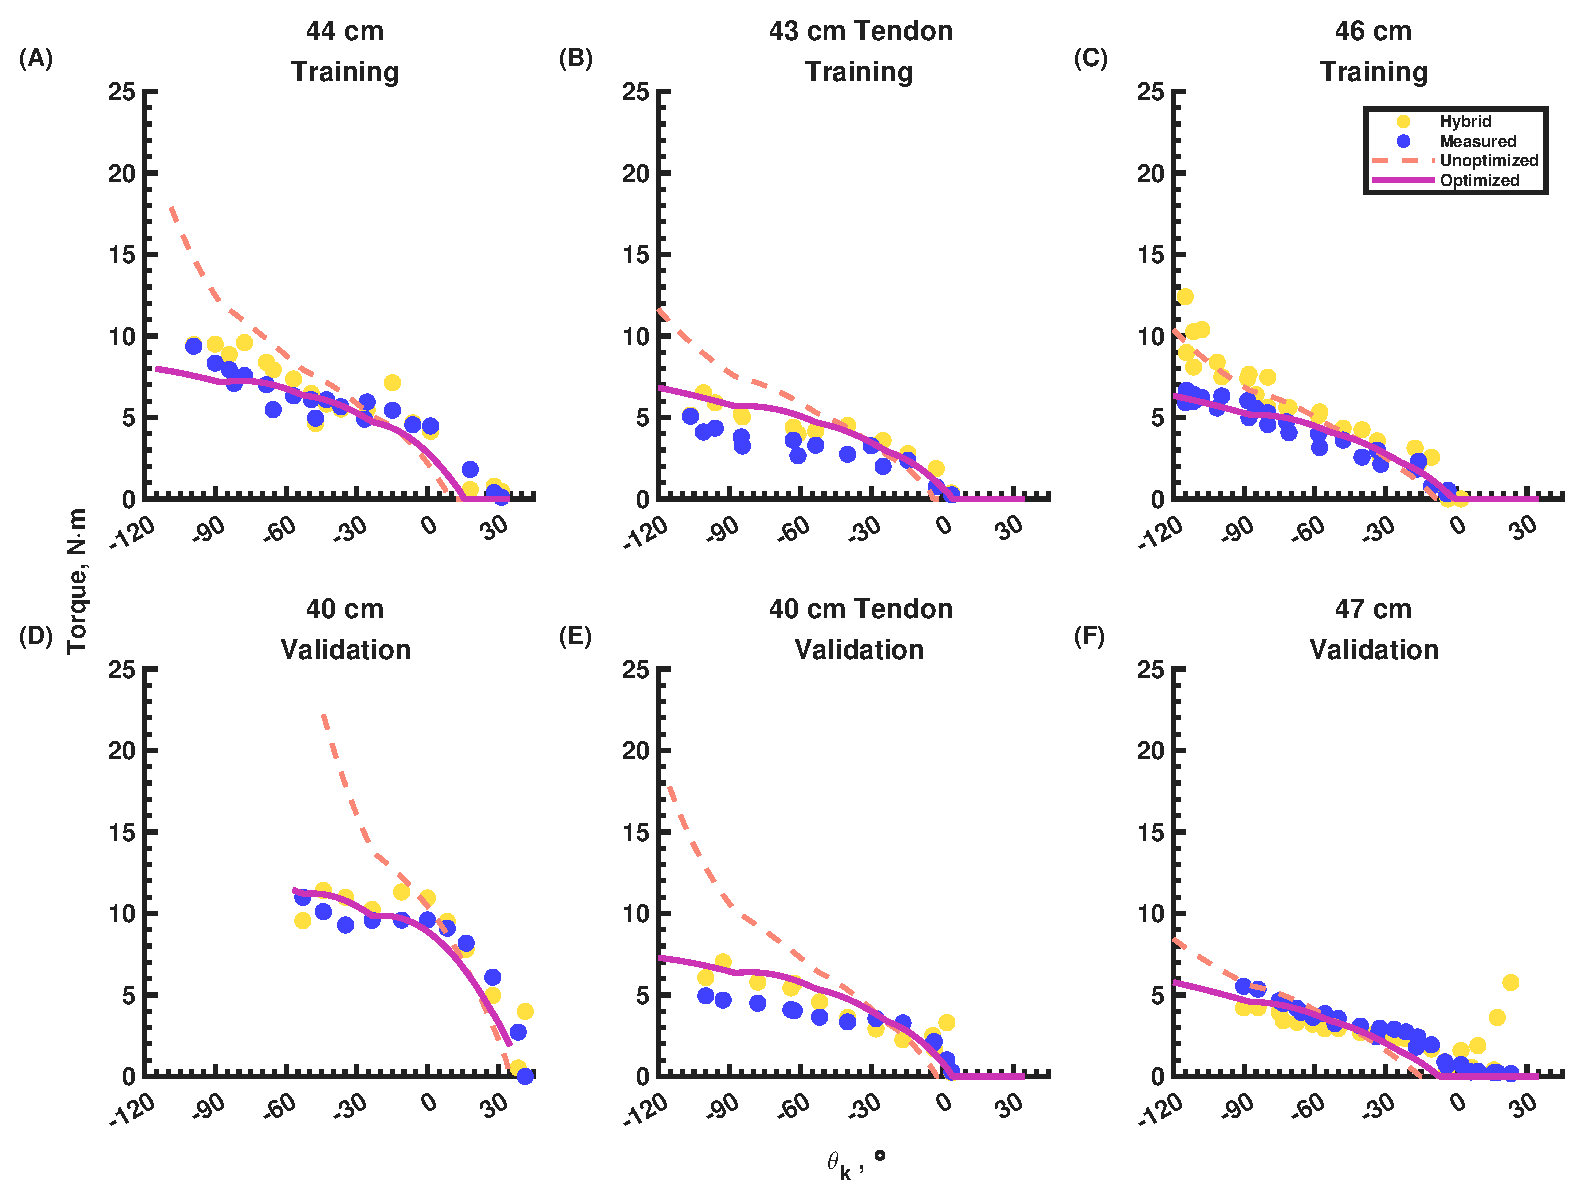
\includegraphics[width=1\textwidth]{ExtPin_group.eps}
\end{center}
\caption{Pinned-knee torque versus knee angle for the extensor BPAs: the six identification-pool tests at the adopted correction terms, with the extensor-specific terms $(\chi_{0}, \chi_{3})$ on the shared stiffness pair (Table~\ref{tab:AdoptedXi}). Knee angle is negative in flexion, and extension torque is positive. Gold circles are the hybrid calculation; indigo filled circles are experimentally measured torque; the dashed light orange line is the unoptimized prediction of the improved BPA characterization; the magenta line is the optimized prediction of the corrected model. Panel titles give the nominal resting length; the actual resting lengths are $l_{0}=\qty{43.6}{\cm}$ \textbf{(A)}, $l_{0}=\qty{43.2}{\cm}$ with tendon \textbf{(B)}, $l_{0}=\qty{45.7}{\cm}$ \textbf{(C)}, $l_{0}=\qty{40.0}{\cm}$ \textbf{(D)}, $l_{0}=\qty{40.0}{\cm}$ with tendon \textbf{(E)}, and $l_{0}=\qty{46.5}{\cm}$ \textbf{(F)}. Panels \textbf{(A)}--\textbf{(C)} are the training tests and panels \textbf{(D)}--\textbf{(F)} the held-out validation tests of the adopted cross-validation fold; the legend is given in panel \textbf{(A)}.}\label{fig:ExtPin_group}
\end{figure}

Results are shown in Fig. \ref{fig:ExtPin_group}. The initial identification was fitted in cross-validated rounds over the \qty{48.0}{\cm}, \qty{45.7}{\cm}, and \qty{41.5}{\cm} actuators, holding each actuator out in turn, and the quoted round is the one holding out $l_{0}=\qty{41.5}{\cm}$; it resulted in $\chi_{0} = \qty{-10.9}{\mm}$ and $\chi_{3} = 0.123$, the extensor length offset $\chi_{0}$ being nearly equal in magnitude to the flexor offset but opposite in sign. The goodness-of-fit values of the initial round are found in Table~\ref{tab:TorqueFit}. The two-stage extensor refit of Section~\ref{sec:identification} used a different six-test pool (Table~\ref{tab:ExtPinGof}) drawn from the same test campaign, in which the \qty{41.5}{\cm} and \qty{48.0}{\cm} tests of the initial set were excluded from the pool and the \qty{45.7}{\cm} test served as a training test of the adopted fold; Fig.~\ref{fig:ExtPin_group} shows the six pool tests at the adopted terms.

At the adopted correction terms of the full re-identification (Section~\ref{sec:identification}), Table~\ref{tab:ExtPinGof} reports the per-test goodness of fit on the six extensor tests used by the identification, three for training and three for validation: the corrected model improves the RMSE of every used test over the zero-correction prediction and holds FVU below unity on all but the $l_{0}=\qty{43.2}{\cm}$ tendon test. The original rigid-body model on these tests is shown graphically in Fig.~\ref{fig:ExtPin_group}.

\begin{table}[htbp]
\caption{Pinned-knee extensor torque-prediction goodness of fit per test, at the adopted correction terms (stiffness pair locked to the flexor-identified values). The zero-correction prediction uses the improved BPA force characterization alone; the corrected model adds the extensor-specific terms $(\chi_{0}, \chi_{3})$. RMSE and maximum absolute residual (Max.) are in $\text{N}\cdot\text{m}$. The extensor terms were trained on the $l_{0}=\qty{43.6}{\cm}$, \qty{43.2}{\cm} tendon, and \qty{45.7}{\cm} tests and validated on the $l_{0}=\qty{40.0}{\cm}$, \qty{40.0}{\cm} tendon, and \qty{46.5}{\cm} tests; the three remaining extensor tests were not used (Appendix~\ref{app:model_geometry}).}
\label{tab:ExtPinGof}
\begin{tabular}{@{}lcccccc@{}}
\toprule
& \multicolumn{3}{c}{\textbf{Improved BPA char.\ alone}} & \multicolumn{3}{c}{\textbf{Corrected model}} \\
\cmidrule(lr){2-4} \cmidrule(l){5-7}
\textbf{Test} & \textbf{RMSE} & \textbf{FVU} & \textbf{Max.} & \textbf{RMSE} & \textbf{FVU} & \textbf{Max.} \\
\midrule
$l_{0}=\qty{43.6}{\cm}$ (training)        & 2.437 & 0.9618 & 4.284 & 0.978 & 0.1634 & 1.818 \\
$l_{0}=\qty{43.2}{\cm}$, tendon (training) & 2.878 & 4.7304 & 4.817 & 1.525 & 1.3270 & 2.481 \\
$l_{0}=\qty{45.7}{\cm}$ (training)         & 2.178 & 1.0586 & 4.974 & 0.490 & 0.0535 & 1.206 \\
$l_{0}=\qty{40.0}{\cm}$ (validation)       & 3.092 & 0.5638 & 4.842 & 1.244 & 0.1303 & 2.196 \\
$l_{0}=\qty{40.0}{\cm}$, tendon (validation) & 3.622 & 6.3919 & 7.845 & 1.350 & 0.8878 & 1.890 \\
$l_{0}=\qty{46.5}{\cm}$ (validation)       & 0.949 & 0.3152 & 2.272 & 0.699 & 0.1714 & 1.559 \\
\midrule
Mean (training)                           & 2.498 & 2.2502 & 4.692 & 0.997 & 0.5146 & 1.835 \\
Mean (validation)                        & 2.554 & 2.4236 & 4.986 & 1.098 & 0.3965 & 1.882 \\
\bottomrule
\end{tabular}
\end{table} 


\subsection{Extensor on Biomimetic Knee}


The biomimetic knee was tested with a $\diameter$\qty{10}{\mm} BPA in the extensor configuration. The bracket frame origin is the centroid of the cantilevered segment that holds the muscle origin bracket to the proximal femur (see Fig. \ref{fig:bktFrame}\textbf{C}, right side).

The torque results for a $l_{0}=\qty{51.8}{\cm}$ BPA are shown in Fig. \ref{fig:Ext10mm_52cm}. The torque values measured are significantly smaller than both the original prediction and back-calculated torque using the hybrid method. The results from the previous extensor configuration lead to a better torque prediction. GoF values can be found in table \ref{tab:TorqueFit}. Fig.\ref{fig:Ext_passthru} shows the difficulty of modeling a BPA path that passes through the femoral condyles. Using the optimization results for extensor BPAs on the pinned knee joint, the $l_{0}=\qty{51.8}{\cm}$ BPA has an $\text{RMSE}=0.8920$, $\text{FVU}=0.3396$, and a maximum absolute residual of $1.4188$.

\begin{figure}[htbp]
\begin{center}
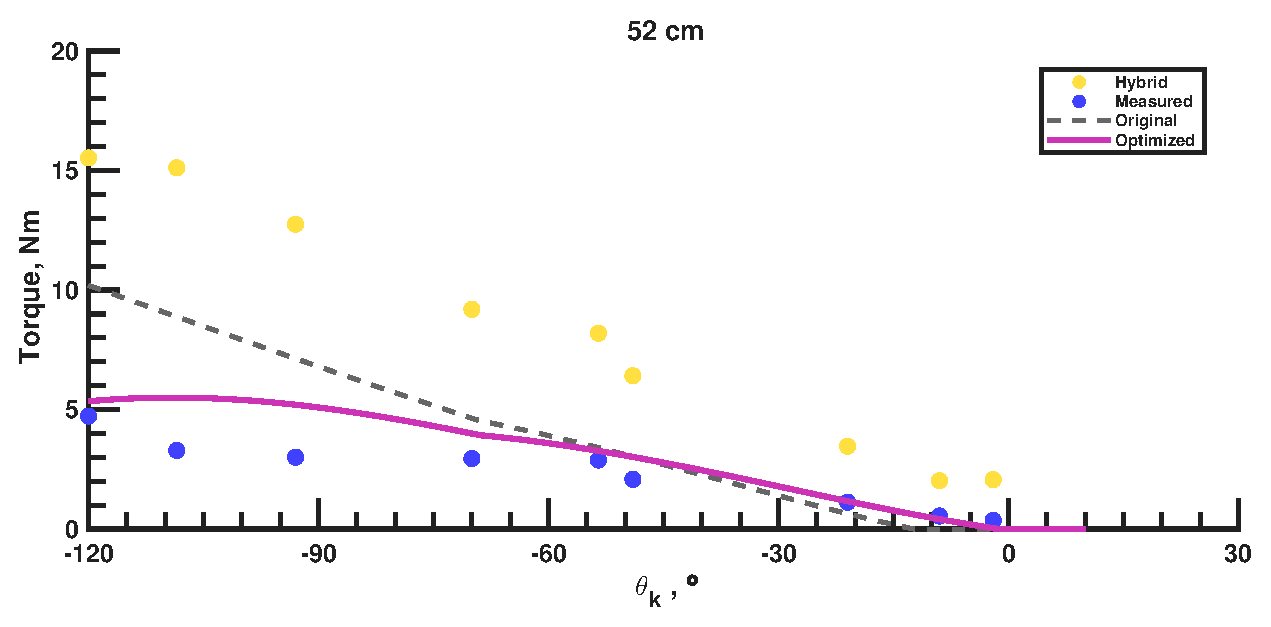
\includegraphics[width=1\textwidth]{Ext10mm_52cm.eps}
\end{center}
\caption{Measured versus expected isometric torque results using a $\diameter$\qty{10}{mm}, $l_{0}=\qty{51.8}{\cm}$ extensor BPA on the biomimetic knee. Measured results are blue dots. Original prediction is a dashed black line. Optimized prediction is a solid magenta line. Hybrid calculation shown in yellow dots.} \label{fig:Ext10mm_52cm}
\end{figure}

\begin{figure}[htbp]
\begin{center}
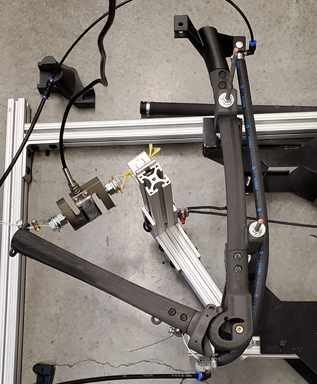
\includegraphics[width=0.65\textwidth]{KneeExt_10mm_passthru.png}
\end{center}
\caption{A configuration that is particularly hard to model. The BPA passes between the femoral condyles close to ICR.}\label{fig:Ext_passthru}
\end{figure}

\subsection{Flexor on Biomimetic Knee}


Fig.~\ref{fig:FlxGrp} shows the biomimetic-knee flexor measurements with the flexor terms carried over unchanged from the pinned-knee identification; the bracket frame for the $\diameter$\qty{10}{\mm} BPA is shown in Fig. \ref{fig:bktFrame}\textbf{C}, and for the $\diameter$\qty{20}{\mm} BPA in Fig. \ref{fig:bktFrame}\textbf{D}. Panel \textbf{A} presents the $\diameter$\qty{10}{\mm} actuator at $l_{0}=\qty{41.5}{\cm}$ with a \qty{21}{\mm} artificial tendon ($\diameter$\qty{1.5}{\mm} Shimano bicycle brake cable wrapped four times), pressurized to \qty{604}{\kPa}; the corrected model reached an RMSE of \qty{0.3007}{\newton\meter}, an FVU of 0.0102, and a maximum absolute residual of \qty{0.4647}{\newton\meter}. Panel \textbf{B} presents the $\diameter$\qty{20}{\mm} actuator at $l_{0}=\qty{41.5}{\cm}$ with a \qty{14}{\mm} artificial tendon made out of the same brake cable, wrapped three times so that six cable segments share the load, each wrap contributing two tendon lengths and cross-sectional areas. Panel \textbf{B} was tested at \qty{620}{\kPa}, for which the corrected model reached an RMSE of \qty{1.8024}{\newton\meter}, an FVU of 0.0499, and a maximum absolute residual of \qty{3.5678}{\newton\meter}.

The torque of the single $\diameter$\qty{20}{\mm} flexor actuator of panel \textbf{B} did not exceed the magnitude of the maximum human isometric flexion torque between \ang{60} and \ang{100} of knee flexion, and within a $\pm 20\%$ band about the human mean it still fell short of human-level torque between \ang{78} and \ang{103} of flexion. Because operating at \qty{620}{\kPa} across the full desired range of motion would load the printed femur beyond its ultimate strength, single points were also recorded at the reduced pressures \qtylist{560;421;325;281}{\kPa}, which show that the desired range of motion is achievable at reduced pressure. This shortfall in flexion torque defines the target that the attachment-route redesign of Section~\ref{sec:ongoing} addresses.

\begin{figure}[htbp]
\begin{center}
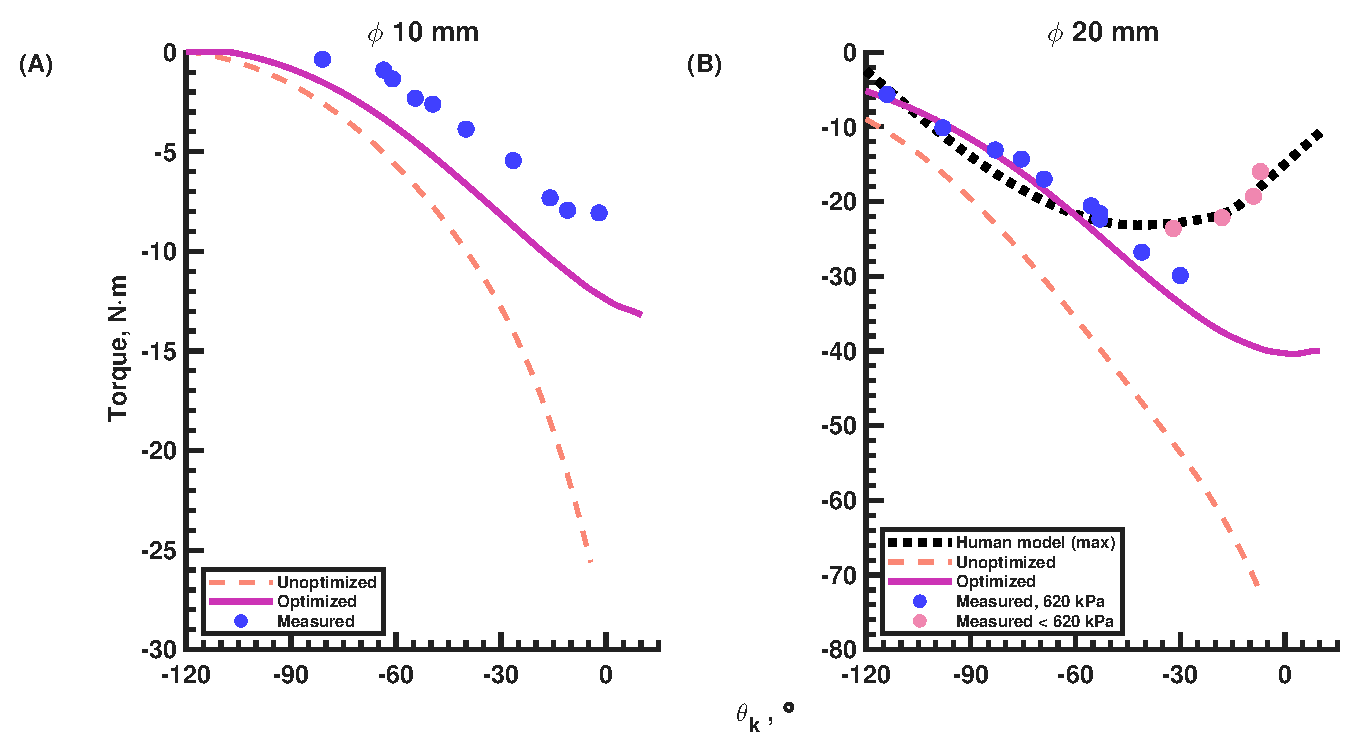
\includegraphics[width=1\textwidth]{FlxGrp.eps}
\end{center}
\caption{Biomimetic-knee torque versus knee angle for the flexor BPAs. Knee angle is negative in flexion, and flexion torque is negative. \textbf{(A)} $\diameter$\qty{10}{\mm}, $l_{0}=\qty{41.5}{\cm}$ actuator with a \qty{21}{\mm} artificial tendon at \qty{604}{\kPa}. \textbf{(B)} $\diameter$\qty{20}{\mm}, $l_{0}=\qty{41.5}{\cm}$ actuator with a \qty{14}{\mm} artificial tendon at \qty{620}{\kPa}. Indigo filled circles are measured torque; the magenta line is the optimized prediction of the corrected model using the flexor terms identified on the pinned knee; the dashed light orange line is the unoptimized prediction of the improved BPA characterization alone. In \textbf{(B)}, the black dotted line is the maximum human isometric torque, and the pink circles are measured points at the reduced pressures \qtylist{560;421;325;281}{\kPa} (from left to right, respectively), recorded because full pressure would load the printed femur beyond its ultimate strength.}\label{fig:FlxGrp}
\end{figure}



\begin{table}[htbp]
\caption{Goodness of fit for the improved torque model across test configurations. RMSE and maximum absolute residual are in $\text{N}\cdot\text{m}$.}
\label{tab:TorqueFit}
\begin{tabular}{@{}lccc@{}}
\toprule
\textbf{Configuration} & \textbf{RMSE} & \textbf{FVU} & \textbf{Max.\ residual} \\
\midrule
Flexor, pin joint, $l_{0}=\qty{48.5}{\cm}$ (training) & 1.616 & 0.0958 & 3.2527 \\
Flexor, pin joint, $l_{0}=\qty{45.7}{\cm}$ (validation) & 2.1214 & 0.0878 & 5.1690 \\
Extensor, biomimetic knee, $l_{0}=\qty{51.8}{\cm}$ & 0.8920 & 0.3396 & 1.4188 \\
Flexor, biomimetic knee, $\diameter$\qty{10}{\mm}, $l_{0}=\qty{41.5}{\cm}$ & 0.3007 & 0.0102 & 0.4647 \\
Flexor, biomimetic knee, $\diameter$\qty{20}{\mm}, $l_{0}=\qty{41.5}{\cm}$ (\qty{620}{\kPa}) & 1.8024 & 0.0499 & 3.5678 \\
\bottomrule
\end{tabular}
\end{table}

\section{Discussion}

\subsection{Sources of Error in Isometric Torque Generation}\label{sec:disc_error}

Our improved BPA characterization predicts torque more accurately than the original BPA model (see Fig.~\ref{fig:FlxPin_preopt}). This only accounts for part of the error. Many factors affect the torque results. Compliance in the testing system, positioning tolerances, flexibility of brackets, imperfect path modeling, and variation in individual BPAs are other factors.

Simplifying and testing the model revealed deficiencies in our previous analysis. The isometric system is not rigid. There is compliance in the winch cable, artificial tendons, and brackets that bend and stretch. We introduced a constant length offset term $\chi_{0}$, axial stiffness $\chi_{1}$, and bending stiffness $\chi_{2}$. The bracket frame of reference was placed at the onset of the cantilevered section and rotated about $Z$.  The optimization identified parameter values for a $\diameter$\qty{10}{\mm} BPA with $l_{0}=\qty{48.5}{\cm}$ in the simple pinned knee configuration. These results were validated with a second $\diameter$\qty{10}{\mm} BPA with $l_{0}=\qty{45.7}{\cm}$.

The modeling of extensor BPA paths that wrap around the knee joint is an approximation with inherent error (Fig. \ref{fig:Ext_passthru}). When the moment arm is short, small changes to it can have a large effect on the resultant torque \citep{young_analyzing_2019}. It was assumed that wrapping the BPA around the joint would be easier to account for than adding a patella, deterministically designing its location as a function of knee angle, and accounting for friction. At greater knee flexion angles, shorter $l_{0}$ BPAs were observed to stretch and compress (see Fig.~\ref{fig:testJigs}\textbf{C}). The same loading sometimes caused the BPA to slip off the anterior head of the bolt that holds the femur to the knee. This produced a \qty{\pm 20}{\mm} displacement in the $Z$ direction, changing both the force vector and the torque. Fig. \ref{fig:ExtPin_group} shows a deviation between measured and originally predicted results that widens as expected torque increases. This indicates system compliance. However, the hybrid-calculated torque matches or exceeds the predicted torque, except at greater flexion angles for the $l_{0}=\qty{41.5}{\cm}$ BPA, indicating a loss of functional $l_m$; this is why the $\chi_{3}$ term was created in \eqref{eq:deltaL}. Fig. \ref{fig:ExtPin_group} shows the improved fit from running the optimization that includes this term.

The biomimetic knee joint with an extensor BPA was used to validate the extensor optimization results. The corrected prediction more closely matches the measured torque values, although it remains higher than the measurements.


The nonlinear biomimetic robotic system presented here replaces rigid-body simplifications commonly used in other robotic and biomechanical systems. Instead, progressing from simple to complex systems elucidated compliance mechanisms that can lead to more accurate first-iteration designs. Technologies have been developed to predict system bending and axial compliance, a constant length offset, and a loss of usable length that occurs as artificial muscle bends around a joint. 

The quasi-static force characterization also fixes the coefficients that a dynamic actuator model needs. Writing the actuator's contraction as a second-order system, $m\ddot \varepsilon^* + c (\dot \varepsilon^* ) \dot \varepsilon^* + k ( \varepsilon^* ) \varepsilon^* = F$, the stiffness term is the tangent slope of the normalized force surface of Equation~\eqref{eq:Fstar}, $k(\varepsilon^{*}, P^{*})
= \left.\frac{\partial F}{\partial \varepsilon^{*}}\right|_{P^{*}}
= -c_{0}c_{1}e^{-c_{1}\varepsilon^{*}}
  - 2c_{2}\varepsilon^{*}P^{*}e^{-c_{2}(\varepsilon^{*})^{2}}$. Setting the mass and the external force to zero then yields the equivalent viscous damping coefficient, $c (\dot \varepsilon^* ) = (k ( \varepsilon^* ) \varepsilon^*)/\dot \varepsilon^*$, the term that dynamic state-space actuator models, such as the pressure--force formulation of \citet{elzein_pressure_2025}, pair with this stiffness.

\subsection{Follow-Up Identification and Route Redesign}\label{sec:ongoing}

The coefficient values reported with the results figures belong to the initial single-bracket identification. Re-identifying the correction terms over the full test sets with the two-stage procedure of Section~\ref{sec:identification} yields the adopted values $\chi_{0} = \qty{+3.94}{\mm}$, $\chi_{1} = \qty{3.998e4}{\N\per\m}$, and $\chi_{2} = \qty{1.473e4}{\N\per\m}$ for the flexor, and $\chi_{0} = \qty{-6.38}{\mm}$ with $\chi_{3} = 0.158$ for the extensor on that same locked stiffness pair (Table~\ref{tab:AdoptedXi}); the search bounds and the adopted values are recorded in Appendix~\ref{app:model_geometry} (Tables~\ref{tab:app_opt_bounds} and~\ref{tab:app_xi_values}).

\begin{table}[htbp]
\caption{Adopted correction terms of the two-stage identification. The extensor refit locked the effective-stiffness pair $(\chi_{1}, \chi_{2})$ to the flexor-identified values, so a single stiffness pair is shared across the flexor and extensor configurations, and only $\chi_{0}$ and $\chi_{3}$ were re-identified for the extensor. The pair was adopted from a family of near-equivalent fits by a requirement external to the identification, namely that both route-redesign configurations meet the required \qty{5}{\percent} torque-overshoot target simultaneously. The stiffness terms are effective system stiffnesses that lump the compliance of the brackets, fixtures, and winch cable; $\chi_{3}$ is unitless and scales the fictive-strain wrapping loss.}
\label{tab:AdoptedXi}
\small
\begin{tabular}{@{}lllp{5.8cm}@{}}
\toprule
\textbf{Parameter} & \textbf{Value} & \textbf{Search bounds} & \textbf{Configuration and role} \\
\midrule
$\chi_{0}$ & \qty{+3.94}{\mm} & \qtyrange{0}{20}{\mm} & Flexor: constant effective-length offset \\
$\chi_{1}$ & \qty{3.998e4}{\N\per\m} & \qtyrange{3e4}{1e6}{\N\per\m} & Flexor: effective axial stiffness (bracket-frame $x$ and $z$) \\
$\chi_{2}$ & \qty{1.473e4}{\N\per\m} & \qtyrange{5e3}{2e4}{\N\per\m} & Flexor: effective bending stiffness (bracket-frame $y$) \\
$\chi_{0}$ & \qty{-6.38}{\mm} & \qtyrange{-20}{5}{\mm} & Extensor: constant effective-length offset (opposite sign to the flexor value) \\
$\chi_{3}$ & \num{0.158} & \numrange{0}{1} & Extensor: wrapping-loss (fictive-strain) scale factor \\
\bottomrule
\end{tabular}
\end{table} The pinned-flexor data do not uniquely determine the stiffness pair, because a family of pairs reproduces the training tests nearly equally well, so the adopted pair was selected by a requirement external to the fit: both redesign configurations must meet the required 5\,\% torque-overshoot target simultaneously. What the correction terms do to the prediction is quantified in Tables~\ref{tab:FlxPinGof} and~\ref{tab:ExtPinGof}. The corrected flexor model holds FVU at or below 0.18 on the four tests of the identification, the worst case being the \qty{48.5}{\cm} training test at 0.172, and the post hoc evaluation of the unused \qty{47.9}{\cm} test improves as well (Appendix~\ref{app:model_geometry}). On the extensor identification the corrected model improves the RMSE on every used test, cutting the training-triple mean from \qty{2.50}{\newton\cdot\meter} to \qty{1.00}{\newton\cdot\meter} and the validation-triple mean from \qty{2.55}{\newton\cdot\meter} to \qty{1.10}{\newton\cdot\meter}, and holds FVU below unity on every used test except the \qty{43.2}{\cm} tendon test. On the biomimetic extensor test ($l_{0} = \qty{51.8}{\cm}$) the corrected prediction improves RMSE from \qty{3.03}{\newton\cdot\meter} to \qty{1.17}{\newton\cdot\meter} and FVU from 4.49 to 0.67, so the shared-pair model explains the bulk of that configuration's measured torque variance as well as its level. The genetic multiobjective solver is retained for the identification, where the Pareto front is required for holdout validation, and the surrogate-plus-pattern-search pipeline serves the route redesign (Section~\ref{sec:optimization}).

The route redesign built on these values addresses the single-muscle shortfall at high flexion angles documented in Section~\ref{sec:results_torque}: each configuration now carries two \qty{20}{\mm} BPAs per route. The flexor solution meets the flexor torque target with a minimum margin of $+5.01$\,\% at $-107^{\circ}$, under the modeling assumption that both actuators share one attachment route rather than a physically mirrored pair; making the mirrored pair explicit is the next design refinement. The direct extensor route meets or exceeds its human-scaled target with the required 5\,\% overshoot as the thinnest margin at every angle, $+5.02$\,\% at worst, while respecting the wrap-release schedule and contraction limits of the route-elimination rule (Appendix~\ref{app:model_geometry}); it was later superseded by the cam redesign of Section~\ref{sec:route_redesign_results}. These redesign solutions are the model definitions carried into the neuromechanical simulation work of Sections~\ref{sec:preliminary_sim_methods}--\ref{sec:preliminary_sim_results} and Chapter~\ref{ch:futurework}.

\subsubsection{Redesigned-Route Results on the Gait2392 Robot-Body Model}\label{sec:route_redesign_results}

This subsection records the quantitative outcomes of the redesigned routes on the Gait2392-derived robot-body model, whose muscle force and torque targets define the redesign objectives. All three result families were produced by the surrogate-plus-pattern-search pipeline of Section~\ref{sec:optimization} under the adopted correction terms (Appendix~\ref{app:model_geometry}, Table~\ref{tab:app_xi_values}) with one shared actuator plan: two \qty{20}{\mm} BPAs per route, a \qty{620}{\kPa} pressure ceiling, and a maximum usable contraction of 0.255 in the force model. Each family minimizes its own objective function, a unitless weighted sum of normalized penalty terms in which zero corresponds to no violated penalty, led by the worst-angle and mean-square torque shortfall against the required 5\,\%-overshoot human envelope, followed by overshoot, rest-length, strain, contraction, and mild design-change penalties. The three functions differ in penalty families and normalizations (the flexor and pulley objectives add off-axis-excess, wrap-release, and second-BPA anchor terms, and the pulley objective evaluates its torque requirement on the insertion-side torque after the tackle's force loss), so their numerical values are not commensurable with one another. The human-scaled requirements are the OpenSim isometric torque profiles of the reference human muscles over the same design-grid angles, the vastus medialis for the extensor and the biceps femoris short head for the flexor.

The direct extensor route exceeds the human envelope in magnitude at every angle, with zero shortfall points: across the design range the predicted two-BPA extensor torque spans \qty{35.45}{\newton\cdot\meter} to \qty{109.4}{\newton\cdot\meter} against the human-scaled requirement of \qty{20.25}{\newton\cdot\meter} to \qty{50.32}{\newton\cdot\meter}, and the required 5\,\% overshoot is consumed as the thinnest margin exactly as designed, at a minimum margin of $+5.02$\,\% at the worst-case angle of $-20.2^{\circ}$.

\begin{figure}[p]
\centering
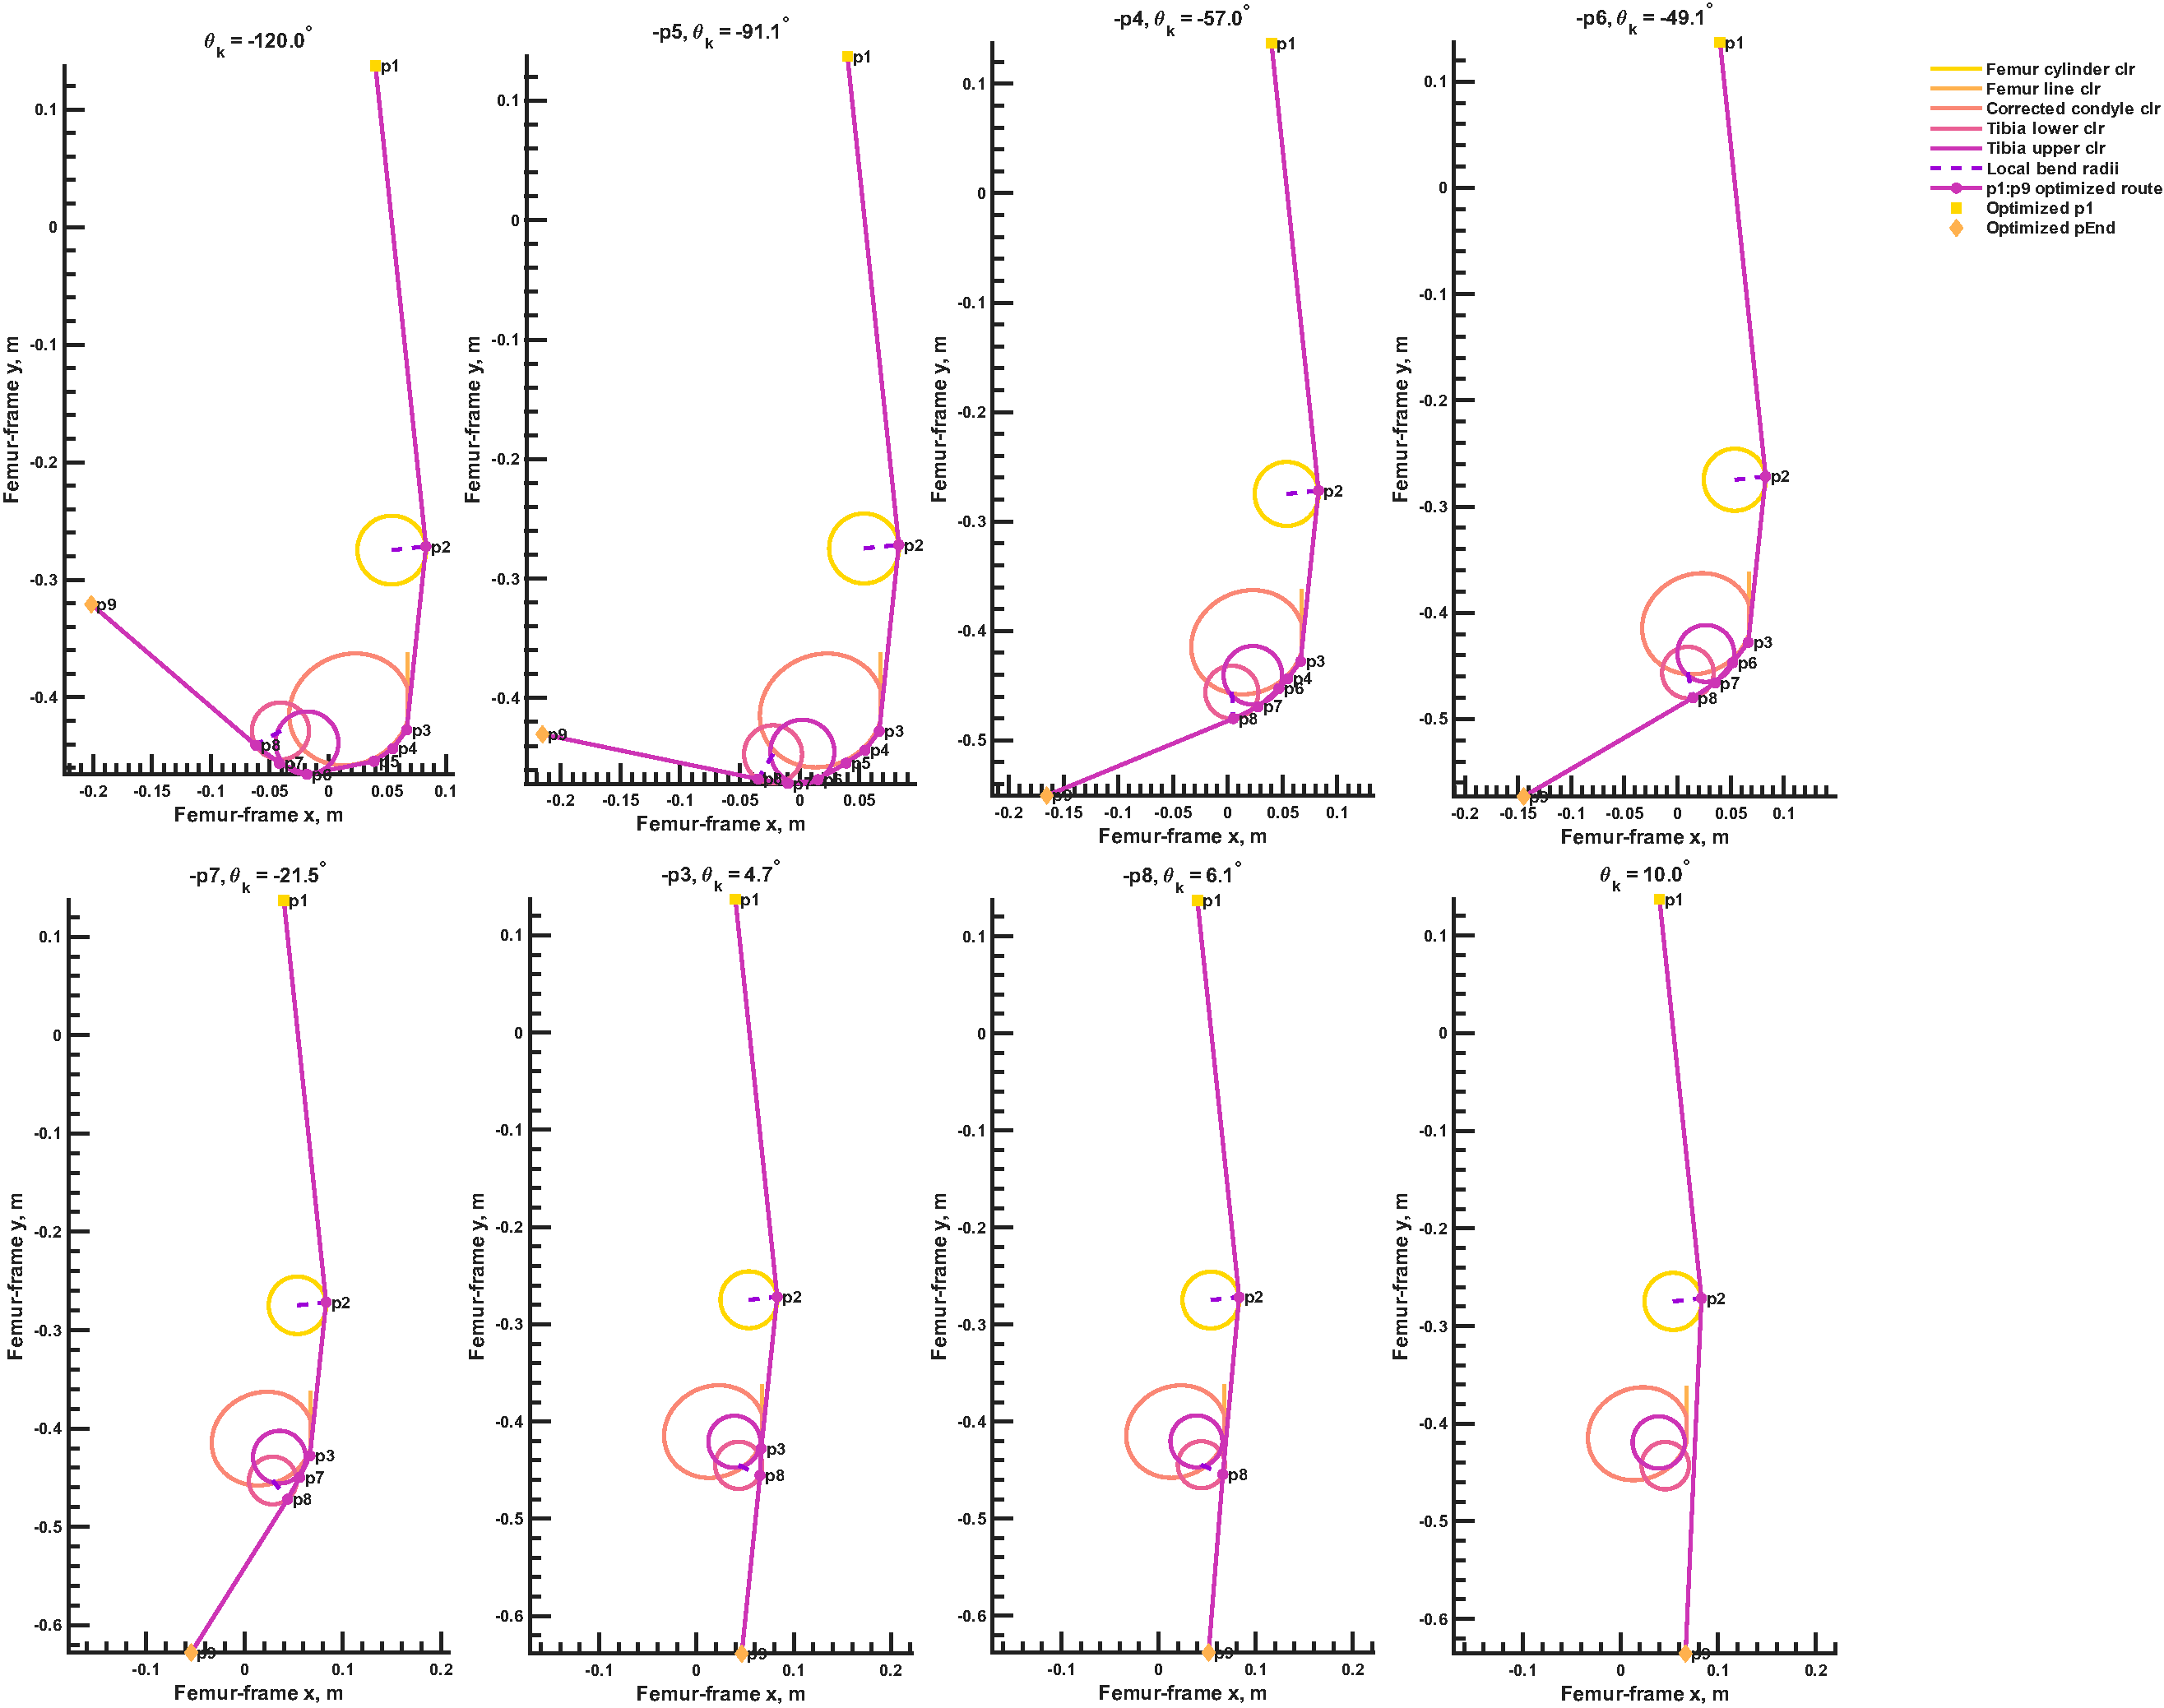
\includegraphics[width=0.98\textwidth]{ExtensorRoute_redesigned.pdf}
\caption[Route geometry of the redesigned extensor route]{Route geometry of the direct extensor route redesign, drawn in the femur frame. Eight pose panels sweep the design range from full flexion ($\theta_\text{k} = \ang{-120}$) through the frame immediately before each of the six contact-elimination events to full extension ($\theta_\text{k} = \ang{10}$); knee angle is negative in flexion. Each panel draws the active route over the femur-cylinder, femur-wall, condyle, and tibia clearance envelopes of the route-elimination rule, with the local bend-radius checks dashed. The square marker is the femur-side origin and the diamond marker is the tibial insertion.}
\label{fig:ExtensorRoute_redesigned}
\end{figure}


The extensor route has since been redesigned once more by allowing the tibial-side route points to trace a cam profile, and this cam redesign is the current extensor design. The cam solution converts the razor-thin margin of the direct route into genuine design headroom. On the final geometry, which folds the optimizer winner together with a verified adjustment of the distal route point and tendon length, the minimum torque margin is $+30.83\,\%$ with respect to the required envelope, the human target plus the 5\,\% overshoot, and $+39.77\,\%$ with respect to the plain human target; the optimizer winner before that adjustment carried $+31.30$\,\% and $+42.34$\,\% at the same checks. The pressure required to meet the envelope spans \SIrange[range-phrase=--]{269}{507}{\kPa} across the range of motion, comfortably above the \qty{150}{\kPa} regulated floor of the VTUG valve manifold that supplies the hardware. The geometry confirms that the headroom is not bought with routing risk: the tibial wrap follows a bend radius of \qty{96.9}{\mm}, the guiding route point clears the femoral-condyle envelope by \qty{43.1}{\mm} at \ang{10} of knee extension, and the moment arm spans \SIrange[range-phrase=--]{59.4}{102.8}{\mm} (mean \qty{72.4}{\mm}) over the range of motion.

The flexor route, built on the same two-BPA arrangement sharing one attachment route, meets the flexor torque target with a minimum margin fraction of 0.0501 against the required 0.05. Its predicted knee-axis torque spans \qty{-81.23}{\newton\cdot\meter} to \qty{-3.864}{\newton\cdot\meter} against the human-scaled requirement of \qty{-23.16}{\newton\cdot\meter} to \qty{-2.461}{\newton\cdot\meter} (peak magnitude \qty{23.16}{\newton\cdot\meter}), again exceeding the human envelope at every angle. The flexor redesign applies the adopted correction terms of Table~\ref{tab:app_xi_values}, including the wrapping factor identified on the extensor configuration.

The Mono/Bi-pulley algorithms extend the route search space by allowing the artificial tendon to be reeved over pulleys before insertion. On the knee-flexor route, the pulley variant converged to a collision-feasible layout with zero bound violations and a peak predicted flexion torque of \qty{85.56}{\newton\cdot\meter} on the insertion-side measure, the torque applied at the insertion after the tackle's force loss; Section~\ref{sec:disc_pulley} quantifies what the redirect adds on the knee-axis measure and the off-axis torque it bounds.

\begin{figure}[p]
\centering
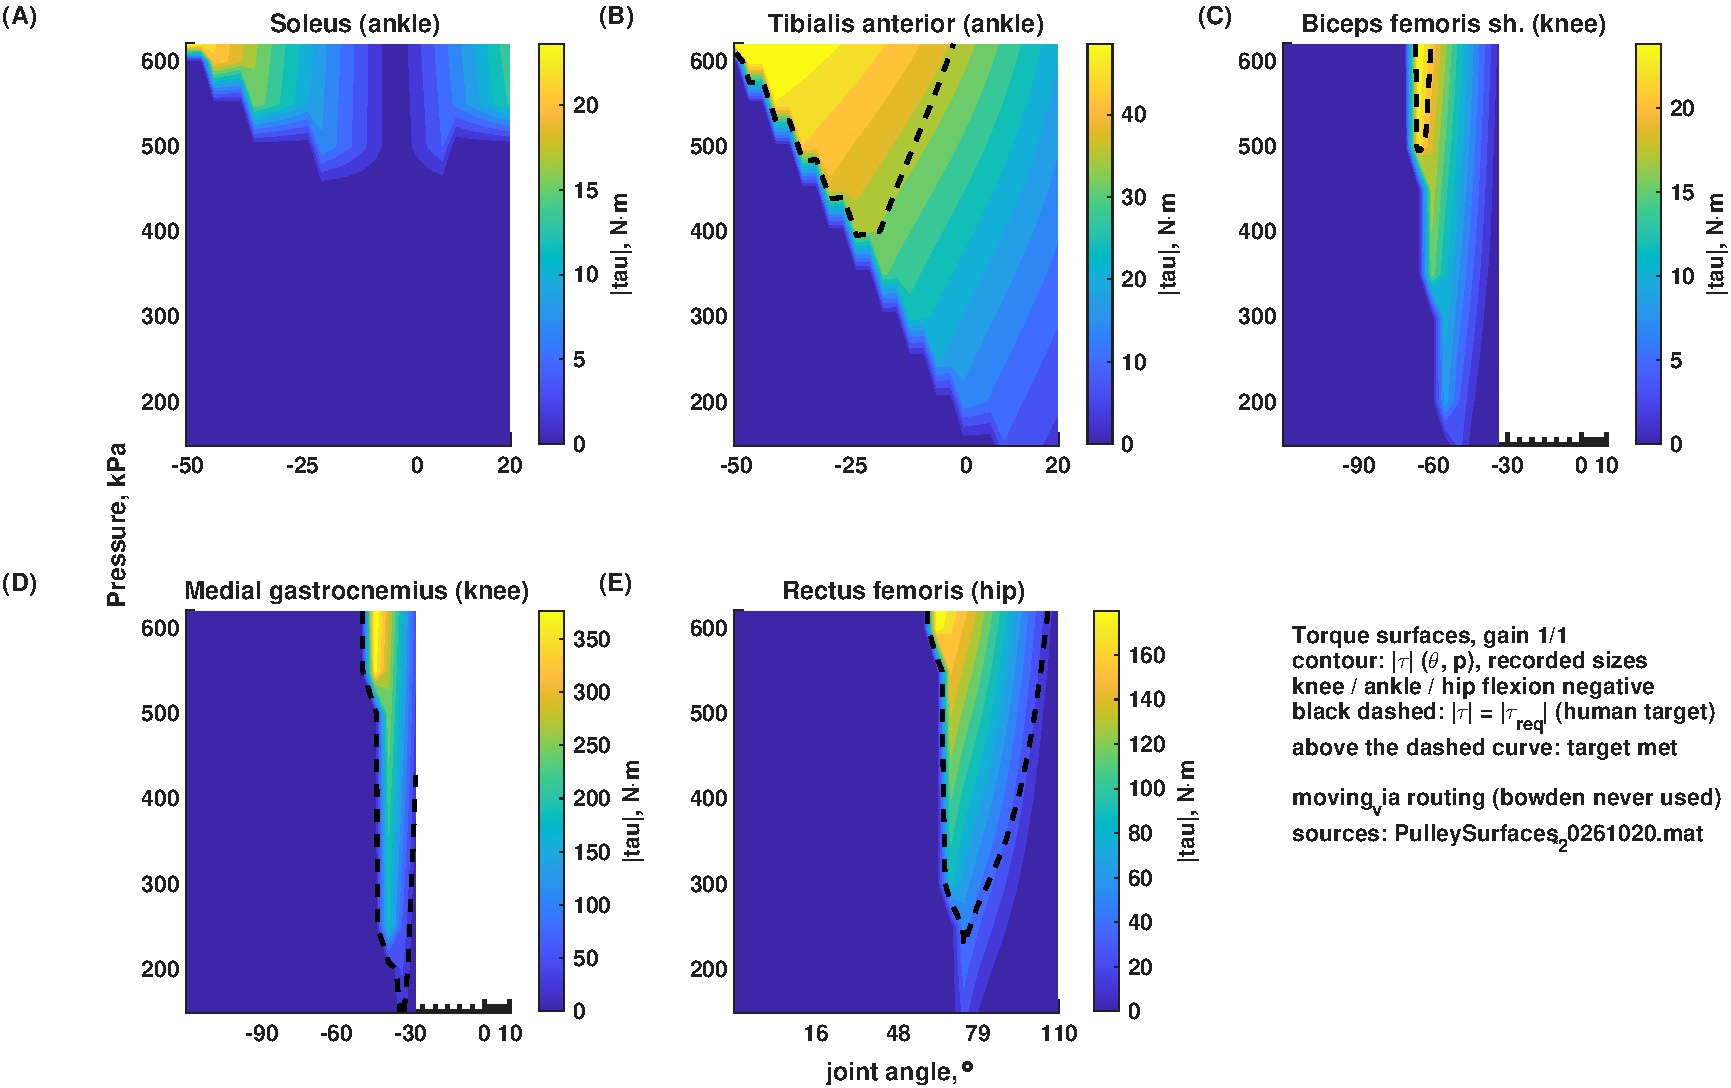
\includegraphics[width=0.98\textwidth]{PulleyTorqueSurfaces_20261020-eps-converted-to.pdf}\par\medskip
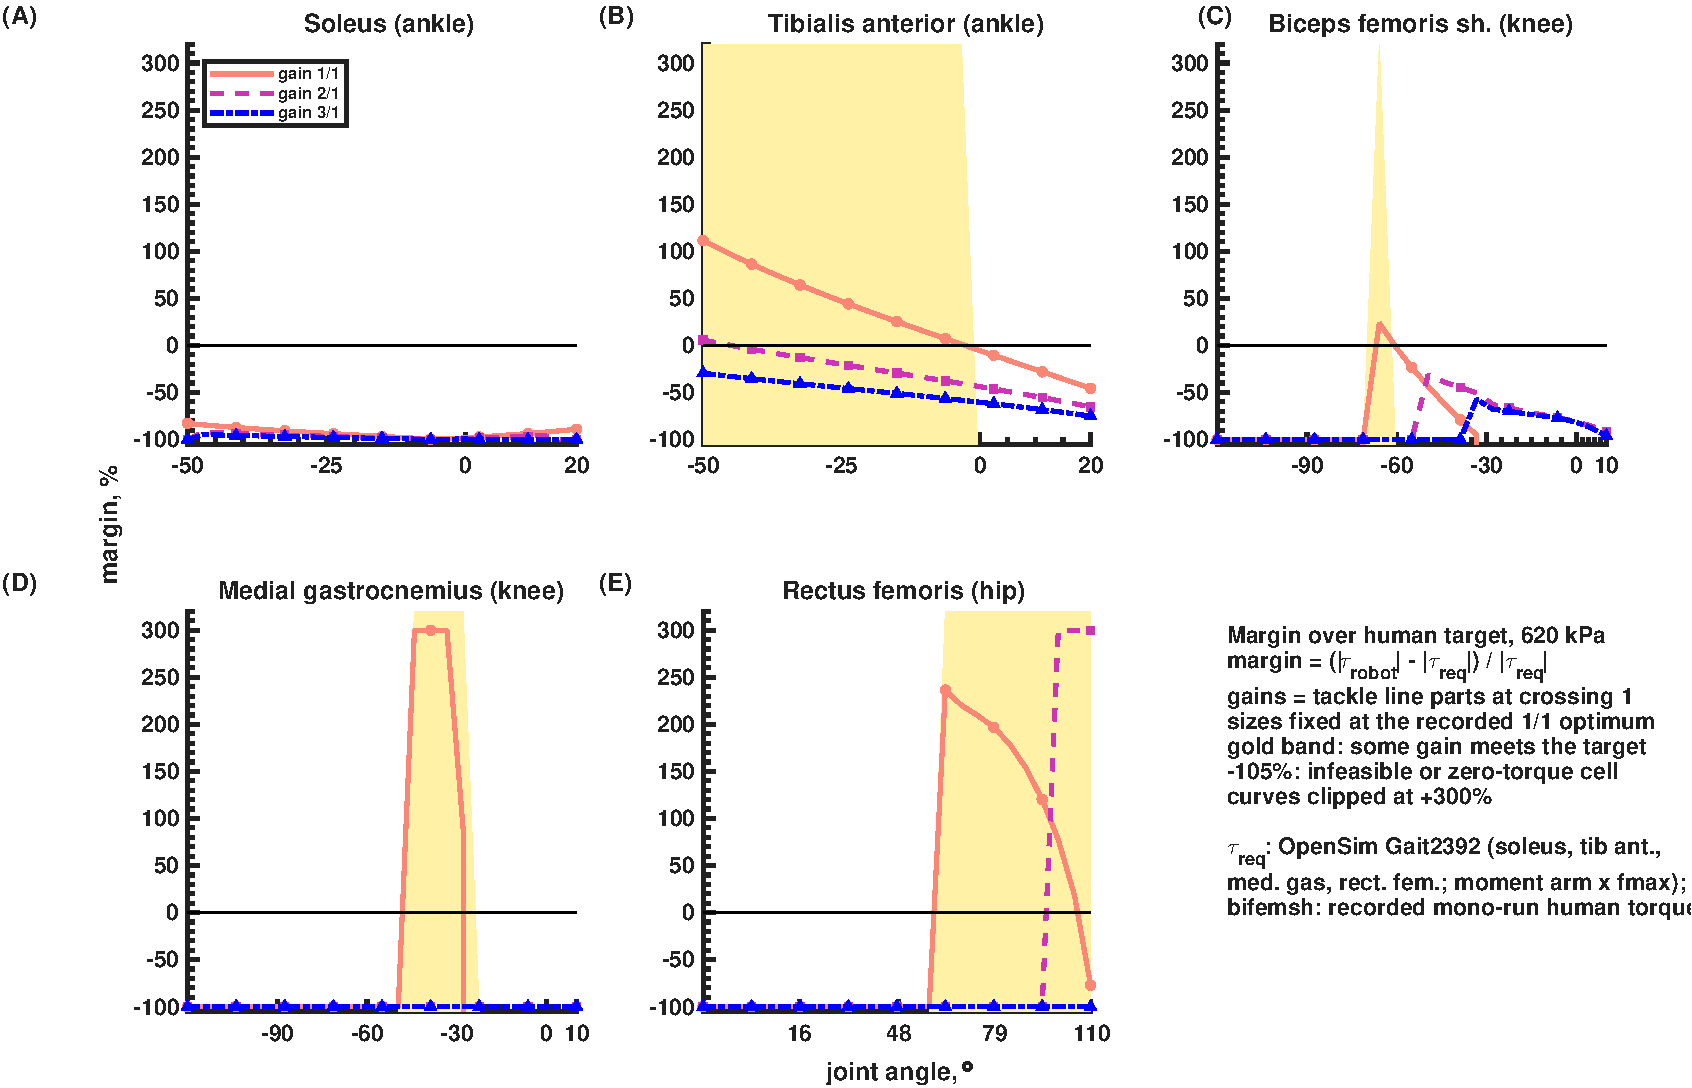
\includegraphics[width=0.98\textwidth]{PulleyMarginSurfaces_20261020-eps-converted-to.pdf}
\caption[Pulley-position sweep surfaces for the reeved flexor route]{Pulley-position sweep for the reeved knee-flexor route. Top: the predicted torque surface over the two pulley positions along the tendon run; bottom: the corresponding torque-margin surface against the human-scaled flexor requirement, on the same position grid. The sweeps show where the reeving freedom pays, the feasible ridges of pulley placement, and where the margin collapses as the geometry approaches the clearance constraints.}
\label{fig:PulleySurfaces}
\end{figure}


The Bi-pulley batch applied the same reeving freedom to five muscle sites of the robot-body model's OpenSim leg, and all five runs failed the torque requirement, with the medial-gastrocnemius and biceps-femoris-short-head runs terminating at the infeasibility sentinel (Table~\ref{tab:bipulley_batch}). For the biceps femoris short head site, whose torque target is \qty{40.2}{\newton\cdot\meter} at the robot-body model's maximum isometric force of \qty{804}{\N}, the pattern search exited with flag $-2$ and returned the sentinel objective of 101 from an initial objective of 1000; Section~\ref{sec:disc_pulley} reports the per-run objectives and the clearance constraints behind these outcomes.

\begin{table}[htbp]
\caption{Bi-pulley batch on five muscle sites of the robot-body model's OpenSim leg. Objective 101 is the batch's infeasibility sentinel; all five runs closed with a nonpositive torque margin. The soleus and tibialis-anterior runs converged feasibly (pattern-search exit flag 1), and their objectives are the normalized torque shortfalls; the remaining three runs exited with flag $-2$.}
\label{tab:bipulley_batch}
\begin{tabular}{@{}lll@{}}
\toprule
\textbf{Muscle site} & \textbf{Objective} & \textbf{Outcome} \\
\midrule
soleus                    & 0.9968                                       & converged (flag 1), nonpositive torque margin \\
tibialis anterior         & 0.9288                                       & converged (flag 1), nonpositive torque margin \\
rectus femoris            & 3.423 (worst constraint 0.2423)              & nonpositive torque margin \\
medial gastrocnemius      & 101, infeasibility sentinel (worst constraint 10) & pattern-search exit flag $-2$ \\
biceps femoris short head & 101, infeasibility sentinel (worst constraint 10) & pattern-search exit flag $-2$ \\
\bottomrule
\end{tabular}
\end{table}

The robot-body model itself carries one update from this work. The adductor magnus attachment point P2 was restored to its full-precision location $(-0.1357, -0.0929, 0.0591)$~m, displacing a rounded copy that was disqualified for producing a zero-length via point that nullified the flexion torque; the regenerated mirrored model passed its validation with zero non-mirrored pairs. At the restored location, the muscle delivers \qty{34.28}{\newton\cdot\meter} of flexion torque, $1.12\times$ the human target of \qty{30.61}{\newton\cdot\meter}, and \qty{27.62}{\newton\cdot\meter} of adduction torque, $0.82\times$ the human target of \qty{33.60}{\newton\cdot\meter}. These redesigned routes remain optimizer-stage results: the robot-body OpenSim model contains no pulley entities, and no via points or markers were added to it for these routes (its eight pre-existing moving-path-point vias, the rectus-femoris and vastii patella-tracking points, one per muscle per leg, belong to the original muscle paths). The MuJoCo conversion used for the simulation work predates the pulley batch and the adductor-magnus restoration, so it carries one stale path point, the pre-restoration rounded adductor-magnus P2. Physical torque tests of the redesigned routes have begun (Section~\ref{sec:disc_pulley}).

The same redesign pipeline was then extended from the knee to all 27 muscle-actuators of the robot-body model, and this whole-body extension is reported as work in progress rather than a completed result. The first pass reached 19 of the 27 actuators before the run stopped, and its chosen solutions showed that the penalty-based formulation itself was the binding limitation: all but one of the chosen routes violated the feasibility constraints, the sole exception being the biceps femoris long-head pair, whose worst-angle margin of $+0.03\,\%$ is indistinguishable from zero. The formulation was then restructured so that the task envelope, the joint-angle window each route must serve, acts as a hard feasible set rather than a penalty. In the restructured pass, twelve of the 27 actuators terminated on a concatenation error in the route builder (the three lumbar-wall actuators, tibialis posterior, the seven distal-foot actuators, and adductor magnus), leaving fifteen finalized routes. Eight of the fifteen were chosen from constraint-feasible configurations: semimembranosus, biceps femoris long head, tensor fasciae latae, soleus, lateral gastrocnemius, tibialis anterior, iliacus, and psoas. Of those eight, six also met the torque requirement at every angle, with worst-angle margins spanning $+0.25\,\%$ (biceps femoris long head) to $+250.7\,\%$ (tensor fasciae latae); the semimembranosus and soleus routes satisfy the geometry but remain short of their torque targets. The crash set and the two torque-short feasible routes define the remaining engineering: the route builder needs a fix for the concatenation failure, and the short routes need either larger actuators or relaxed corridors.

\subsection{Mono- and Bi-Pulley Tendon Routing}\label{sec:disc_pulley}

The route redesign of Section~\ref{sec:ongoing} placed both \qty{20}{\mm} actuators on direct attachment routes. The Mono/Bi-pulley algorithms extend that search space by allowing the artificial tendon to be reeved over pulleys before insertion, and the flexor pulley run quantifies what the added routing freedom is worth on the knee-flexor route. The pulley variant converged to a collision-feasible layout with zero bound violations (pattern-search exit flag 1) at an objective of 0.08465 under its own objective function, which differs from the direct route's objective of 74.47, so the two values are not commensurable. The best configuration on file reeves the two actuators over a single tackle-line part at a gain fixed at 1:1, so the pulley acts as a redirect rather than a force multiplier; even so, the redirect alone deepened the peak predicted flexion torque from \qty{81.23}{\newton\cdot\meter} to \qty{85.74}{\newton\cdot\meter}, a gain of \qty{4.51}{\newton\cdot\meter} (\qty{5.6}{\percent}), while holding the off-axis torque to at most \qty{0.803}{\newton\cdot\meter}, under \qty{1}{\percent} of the peak on-axis value; the predicted peaks of the direct and pulley routes exceed the human flexor torque scale of \qty{23.16}{\newton\cdot\meter} by factors of 3.51 and 3.70. The Bi-pulley batch establishes where that freedom runs out on anatomical routes. Across the five OpenSim muscle sites attempted (soleus, tibialis anterior, rectus femoris, medial gastrocnemius, and biceps femoris short head), every run closed with a nonpositive torque margin (objectives of 0.929 for tibialis anterior, 0.997 for soleus, and 3.42 for rectus femoris with a residual worst-constraint value of 0.242), and the medial-gastrocnemius and biceps-femoris-short-head runs terminated at the infeasibility sentinel (objective 101, worst-constraint value 10, exit flag $-2$). For the four runs that report a finite route-to-route clearance, the binding constraint was geometry rather than torque: minimum pair clearances spanned \qty{4.26}{\mm} to \qty{19.14}{\mm} against the \qty{25}{\mm} separation required between adjacent routes (two \qty{10}{\mm} actuator radii plus a \qty{5}{\mm} bundle margin); the medial-gastrocnemius run records no finite clearance, so its failure rests on the infeasibility sentinel alone. What the two algorithms buy is therefore reach and screening: the mono-pulley converts routing freedom into \qty{4.51}{\newton\cdot\meter} of additional predicted flexion torque without mechanical advantage and with off-axis torque below \qty{1}{\percent} of the peak, and the bi-pulley sweep screens candidate anatomical sites, showing that its reeved routes do not yet fit these corridors and redirecting the design effort toward clearance-relaxed attachment sites. These pulley solutions are optimizer-stage results; they have not yet been propagated into the OpenSim or MuJoCo model trees used for the simulation work of Sections~\ref{sec:preliminary_sim_methods}--\ref{sec:preliminary_sim_results}, and the hardware torque tests of the updated compliant system have begun with the extensor route.

The first physical torque measurements of the redesigned extensor route have been collected. In the first test of the $\diameter$\qty{20}{\mm} extensor on the rebuilt route, three isometric points were held near full extension: measured knee torque of \qty{1.163}{\newton\cdot\meter} at a knee angle of \ang{10}, \qty{7.849}{\newton\cdot\meter} at \ang{11}, and \qty{23.437}{\newton\cdot\meter} at \ang{10}, against hung loads of \qtylist{3.7;25.2;76}{\newton} at gauge pressures of \qtylist{388.5;388;592}{\kPa}, respectively. The first and third points sit at essentially the same knee angle and span a twentyfold range of held torque, so they begin to map the route's response near extension as pressure and load vary. These three points are the start of the torque-versus-angle validation of the redesigned route against its required envelope; the full sweep, and the corresponding flexor measurements, are pending.


